% !TEX root = AImath.v4.tex

\chapter{从传统机器学习到深度学习}
%% 神经网络的发展脉络
% 章节架构
%为什么机器学习方法（如决策树、SVM、逻辑回归等）有局限性？
%为什么引入神经网络？神经元模型如何工作？
%如何从感知机模型发展到前馈神经网络（FNN）？
%神经网络的学习过程（前向传播 + 反向传播 + 梯度下降等）。
%这里的重点是前馈神经网络（FNN）及其学习机制，不深入介绍 CNN、RNN、生成模型等更复杂的架构。

%  从机器学习到深度学习 
 %	1.2.1 智能如何产生：生物神经元的启发  
%      从生物神经元到人工神经网络：深度学习的启发  
%     1.2.2 M-P模型 ： 人工神经网络的雏形  
%	1.2.3 感知机：人工神经网络的起点  
%     多层感知机：从线性到非线性  
%	1.2.4人工神经网路：从简单到深度、多层感知机网络 
%1.3万能逼近定理；
%1.5. 没有免费的午餐定理 6.

\begin{flushright}
“如果我们想创造智能机器，模仿大脑是最自然的路径。” \\
—— 麦卡洛克（Warren McCulloch）
\end{flushright}

在信息爆炸的时代，数据已然成为新的“石油”，而机器学习的使命，就是从这片数据海洋中提炼模式，挖掘其中的潜在规律。近年来，深度学习作为机器学习的一个重要分支，在语音识别、图像分类、自然语言处理、自动驾驶等领域取得了突破性进展，展现了惊人的应用价值。

深度学习的成功秘诀是什么？简单来说，它依赖于三个关键因素：
\begin{itemize}
\item  {\bf 大规模数据：} 数据越多，模型的学习效果越好。就像一个见多识广的老侦探，比新手更容易识破复杂案件的真相。
\item {\bf 高性能计算：}没有强大的计算资源，深度学习的庞大网络就像一辆缺少燃料的赛车，跑不起来。
\item {\bf 深层神经网络的强大学习能力：}深度学习之所以“深”，正是因为它能层层递进，从细节推演整体，像一位善于归纳的学者，从海量信息中自动萃取关键特征。
\end{itemize}

\section{从机器学习到深度学习}
在传统机器学习中，模型学习前需要经过{\bf 人工特征工程（Feature Engineering）}，由专家手动提取如颜色、边缘、形状等特征，再交由分类器进行学习。这种方法虽然有效，但存在两个主要问题：
\begin{itemize}
    \item \textbf{高度依赖人为经验}：特征选取的好坏直接影响模型效果，且不同任务需要不同的特征工程，耗时耗力。
    \item \textbf{难以扩展}：面对海量数据和复杂任务，人工构造特征的方式就像是用算盘计算大数据，效率低下，根本跟不上时代的发展。
\end{itemize}

而\textbf{深度学习的最大突破}在于它利用\textbf{多层神经网络}自动从数据中学习特征，从低级模式（如边缘、纹理）逐步构建高级概念（如猫、狗），跳过传统机器学习中繁琐的特征工程步骤，直接从高维复杂数据（如图像、语音、文本）中提炼信息，大幅提升模型的泛化能力。

\subsection{从人工筛选到自动归纳}

机器学习的发展可以类比于人类识别世界的方式。 传统机器学习像一位依赖手册的侦探，需要有人告诉它该找什么特征，比如“猫的耳朵是尖的，狗的嘴巴较大”。
而深度学习像一位神探，通过自己观察和分析，自动归纳出哪些特征最关键，不再依赖人类给出固定规则。

在传统机器学习中，特征提取和分类为是两个独立的步骤，需要人为拆分任务。而随着数据量的爆炸增长，人工特征提取的效率开始捉襟见肘。

相比之下，以卷积神经网络(CNN)为代表的深度学习提供了另一种“端到端（end-to-end）”的学习范式。这里的“end-to-end”（端到端）是指，输入原始数据（始端），输出最终目标（末端），不再人为拆解子问题，如图~\ref{传统模式分类与深度神经网络的区别与联系}所示。

\begin{figure}[htbp]
\centering
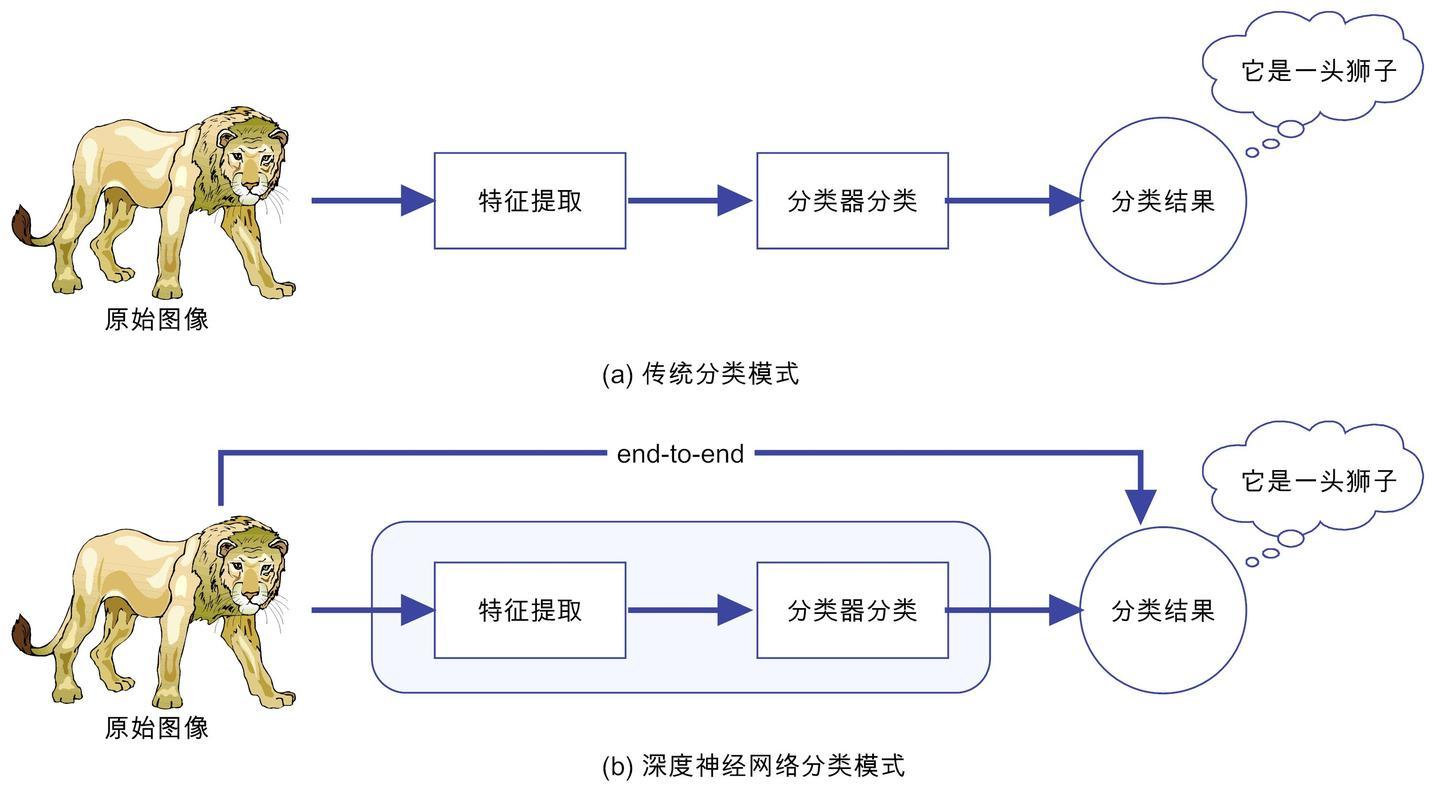
\includegraphics[width=1\textwidth]{figs/传统模式分类与深度神经网络的区别与联系.jpg}
\caption{传统模式分类与深度神经网络的区别与联系}
\label{传统模式分类与深度神经网络的区别与联系}
\end{figure}

\textbf{深度学习通过端到端的训练，让模型从原始数据直接学习映射到最终任务目标}，避免了繁琐的手工特征工程，使得模型更具\textbf{泛化能力}和\textbf{适应性}。

\subsection{从“人工扶持”到“自主学习”}
\subsection{像侦探一样找线索}
想象你是一名侦探，手里有一堆线索（数据）。\textbf{传统机器学习}的方式类似于人工筛选线索——工程师手动挑选最关键的特征，例如，在图像识别任务中，他们可能会精心挑选边缘、颜色、形状等特征，然后交给模型去学习这些特征之间的关系。

但问题在于，{\bf 人类选特征的方式太主观了！} 如果人为定义的规则不够全面，机器在面对新的情况时就会“失灵”——比如，一只耳朵有缺口的猫，传统模型可能无法正确识别。

深度学习换了一种思路——让机器自己找线索。神经网络通过多层学习，逐级提炼特征，就像一个经验丰富的侦探，从零碎的线索中推理出整个案件。

换个角度理解，
\begin{itemize}
    \item 传统机器学习：手工挑选特征，就像老师在考试前划重点，选对了才能考高分。
    \item 深度学习：让学生自己归纳做题方法，不用依赖老师划重点，学得更透彻。
\end{itemize}

\subsection{学骑自行车的启示}
还记得小时候学骑自行车的经历吗？一开始，你可能需要家长扶着，甚至装上辅助轮。经过反复练习，你终于找到了平衡，开始稳稳地骑行，甚至可以轻松应对各种路况。

这和人工智能的成长路径如出一辙：传统机器学习需要人工扶持（特征工程），就像学骑车时家长在旁边扶着。
深度学习则学会了自己掌握平衡，逐渐适应各种复杂任务。

以“猫”和“狗”的图像分类任务为例，在传统机器学习中，工程师需要告诉计算机：“看耳朵形状、毛发颜色、体型大小”来区分猫和狗。而当深度学习见过成千上万张猫和狗的照片后，会自己总结出哪些特征最有区分度，比如：喵星人的耳朵更尖，汪星人的嘴巴更大，甚至可能发现狗通常比猫更爱笑（很多狗的嘴角上扬，看起来像在微笑）。

%这就是深度学习相较于传统机器学习的最大突破：
%\begin{itemize}
%\item \textbf{自动学习特征}：无需人工挑选特征，神经网络自己从数据中提炼模式。
%\item \textbf{端到端训练}：无需人工拆解任务，输入原始数据，输出最终决策，模型自动优化整个过程。    
%\item \textbf{多层级抽象能力}：深度学习能从低级特征（比如线条和颜色）一路学习到高级概念（比如“这是一只猫”），就像写作文，从遣词造句到段落结构，层层递进。
%\end{itemize}

\subsection{ 深度学习的“洋葱式思考”}
深度学习，顾名思义，就是一个 “更深”的神经网络。其核心在于\textbf{层级式特征表示}---从浅层特征（如图像中的边缘）逐步学习到深层语义特征（如图片中的物体类别）。这一特性使深度学习在处理高维复杂数据时具有独特的优势。

想象一下，当你观察一张猫的照片时，会先从局部细节感知，再整合形成完整认知。
你的认知过程大致如下：
\begin{itemize}
   \item 你先注意到边缘和线条（“哦，这里有个轮廓”）。
  \item 然后，你识别出形状和局部特征（“这像是耳朵，这里是眼睛”）。  
  \item  最后，你得出结论：“这是一只猫！”
\end{itemize}

深度学习的工作原理也与此类似---底层学会边缘检测，中层识别局部结构，高层最终判断物体类别：
\begin{itemize}
    \item \textbf{第一层（基础感知）}：提取最基础的边缘、线条、颜色等特征，类似于刚学会画画时画的“毛毛虫线”。
    \item \textbf{第二层（模式识别）}：组合这些特征，形成更具结构性的局部信息，比如眼睛、鼻子、耳朵。
    \item \textbf{第三层（高阶概念）}：综合所有特征，最早判断整张图片的类别，比如“猫”或“狗”。
\end{itemize}

%这就是深度学习的“套路”！ 通过层层提炼，它能从简单的低级特征（比如像素点）逐步理解高级概念（比如一只猫的轮廓）。

\subsection{深度学习为何如此强大？}
\subsubsection{ 超强泛化能力}
深度学习的神奇之处不仅仅是能学会找特征，更在于它的“自适应”能力。

试想一下，一个人如果学习新技能，每次都需要从头来过，那未免太低效了。而深度学习可以借助\textbf{迁移学习（Transfer Learning）}，让一个训练好的模型迅速适应新的任务。

比如，一个训练好的猫狗识别模型，只需稍作调整，就能用于汽车品牌识别；又如，一个普通照片分类模型，可以扩展用于医学影像分析，识别癌细胞。
这种“举一反三”的能力，让深度学习成为人工智能领域里的“最强大脑”。

\subsubsection{ 数据越多，模型越强}
传统机器学习面对大规模数据时太大时容易崩溃，而深度学习则表现出数据越多，模型越强的特性。例如，早期语音识别系统需要大量手工调试，而深度学习的语音识别模型，只要有足够数据，就能自动优化，越来越精准。传统图像分类在数百万张图片上表现一般，而深度学习在百万、甚至亿级别数据集上仍能不断提升。

这就是深度学习相较于传统机器学习的最大突破：
\begin{itemize}
\item \textbf{自动学习特征}：无需人工挑选特征，神经网络自己从数据中提炼模式。
\item \textbf{端到端学习}：无需人工拆解任务，输入原始数据，输出最终决策，模型自动优化整个过程。    
\item \textbf{多层级抽象能力}：深度学习能从低级特征（比如线条和颜色）一路学习到高级概念（比如“这是一只猫”），就像写作文，从遣词造句到段落结构，层层递进。
\end{itemize}

深度学习的崛起，不仅仅是技术的进步，更是人工智能发展史上的一次范式变革。它让计算机从“被动学习”走向“主动探索”，让模型不仅能“做对题”，更能“学会思考”。

\section{生物神经元的启发：模拟大脑}
%\section{深度学习的进化之路：从“模拟大脑”到“突破极限”}
深度学习的历史发展，可以看作是一场不断逼近“智能化”的旅程。从最早的生物神经元研究，到人工神经网络的兴起，再到如今大型神经网络的惊人表现，这条道路充满了挑战与突破。理解其发展脉络，不仅能帮助我们更清楚地认识深度学习的本质，也能洞察人工智能未来的可能性。

如果说深度学习是一座{\bf 摩天大厦}，那么它的地基便是{\bf 人工神经网络（Artificial Neural Networks, ANN）}。

%那么，深度学习是如何一步步走到今天的？它的核心技术有哪些？
在本节中，我们将从深度学习的生物学启发出发，揭示它从理论探索到实际应用的关键突破，如何从最早的单个神经元模型进化到如今的超大规模人工智能系统。

\subsection{深度学习的起源：向人脑学习}
%它模仿了人类大脑的构造和功能，用数学的方法重现了神经元之间传递信号的机制。说白了，深度学习就是试图让机器尽可能靠近生物神经网络的聪明才智。
深度学习出现并非一蹴而就，而是沿着模仿人类智能的路径，一步步演化而来。
想想看，人类是怎么变聪明的？无非是观察世界、提炼规律、然后找到解决问题的方法。
%深度学习{\bf 正是沿着这条“智能之路”，从大量数据中学习模式，再将其应用到现实任务中}，比如看图识猫、帮你推荐下一首最喜欢的歌，甚至陪你打《英雄联盟》。听起来是不是很厉害？
“人法地，地法天，天法道，道法自然。”老子在《道德经》中所阐述的哲思，形象地体现了人类技术发展的灵感来源：效法自然。
自然界的规律为人类提供了无穷无尽的灵感：从蝙蝠声呐导航的研究中，人们获得了发明雷达的灵感；从鱼鳔的启迪下，人们设计了潜水艇......同样，要让“人造物”具备类似人类的智能，模仿人类显然是最直接的路径。

自古以来，人们便认识到智能是大脑生理活动的产物，科学家因此将研究目光投向了大脑。研究大脑的工作原理，用数学的方法模拟这种能力，成为了实现人工智能的理想途径。
%人工神经网络（Artificial Neural Network，ANN）正是在这种探索中应运而生。它是一种模仿动物神经网络行为特征的算法模型，其核心在于通过分布式并行处理，实现复杂问题的求解。

%深度学习通过多层非线性变换，逐步提取数据的潜在模式，解决了传统机器学习对手工设计特征的依赖问题，为语音识别、图像分类、自然语言处理等领域带来了革命性的进展。

%深度学习的发展，是人工智能不断逼近“智能化”的历程。它从最初的“专家规则”走向了“自我学习”，让机器不仅能“做对题”，更能“学会思考”。

\begin{figure}[htbp]
\centering
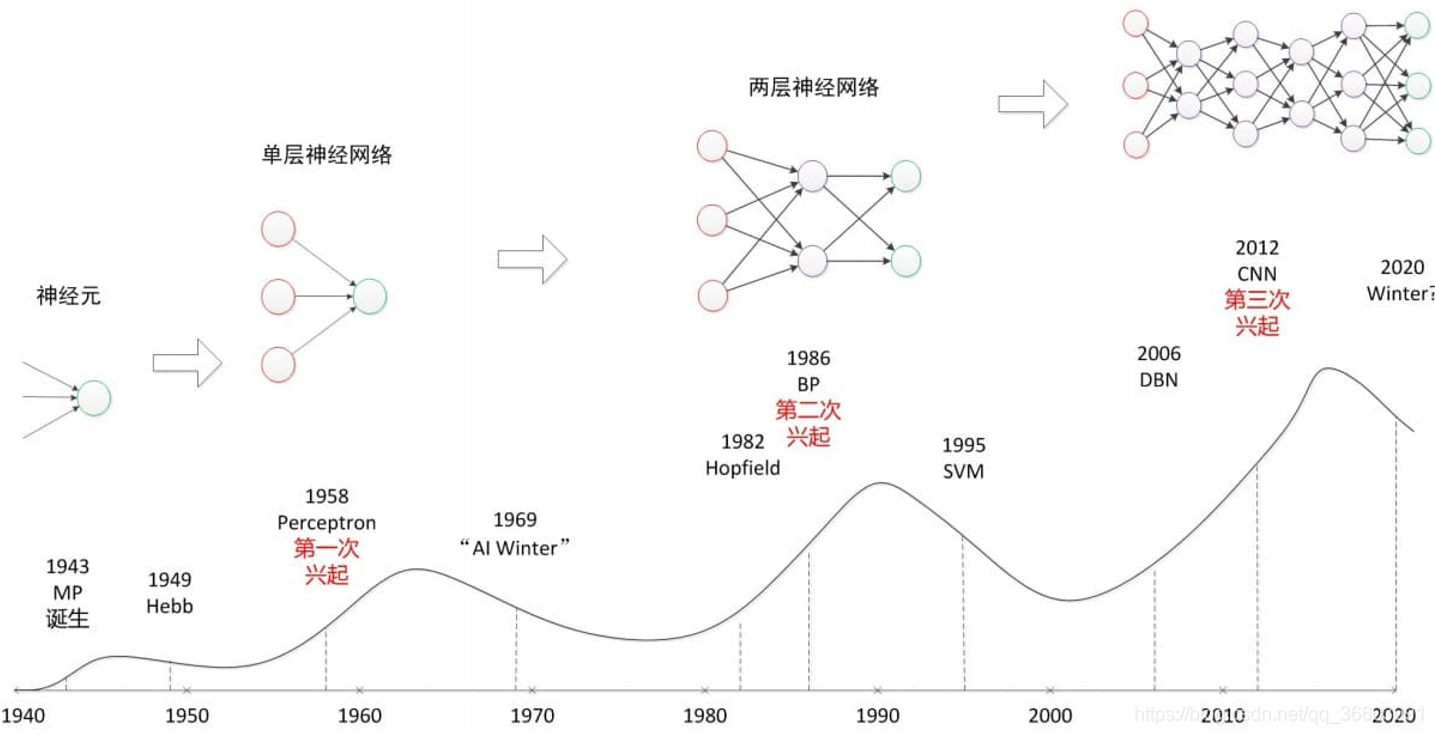
\includegraphics[width=1\textwidth]{figs/ANN.png}
\caption{人工神经网络发展史}
\label{ANN}
\end{figure}

\subsection{智能如何产生：生物神经元的启发}
人工智能的灵感来源于大脑的工作机制，而深度学习更是直接借鉴了生物神经元的信息处理方式。
理解人工神经网络（Artificial Neural Network, ANN）的发展，需要先从其生物学原型——大脑的基本单元神经元（Neuron） 说起。

%\subsubsection{生物神经元：大脑的信息处理单元}

19 世纪末，西班牙科学家 Santiago Ram\'{o}n y Cajal 通过显微镜观察到，大脑由独立的神经元构成，并提出了神经元学说（Neuron Doctrine），奠定了现代神经科学的基础。这一发现首次揭示了大脑的信息处理方式，使得后来的科学家得以研究神经元之间的信号传递机制。%，并为人工神经网络的诞生提供了重要启示。”

人类大脑是一个高度复杂的生物信息处理系统，由约 1000 亿个神经元（$10^{11}$ neurons） 组成，这些神经元通过突触（Synapse）相互连接，形成一个庞大的神经网络，使我们能进行{\bf 感知、学习、记忆、思考和决策}。整个大脑的突触连接数高达$10^{14}$ ，远超过现代计算机芯片的晶体管数量。

尽管单个神经元的结构简单，但其功能强大。它由以下三个主要部分组成(如图~\ref{大脑神经细胞的工作流程} 所示）：
\begin{enumerate}
\item {\bf 细胞体（Soma）：} 神经元的核心部分，整合来自多个突触的输入信号，并决定是否产生新的神经冲动。
\item {\bf   树突（Dendrite）：}接收其他神经元通过突触传递来的电信号，相当于“天线”。
\item {\bf  轴突（Axon）：} 将信号传输到其他神经元，末端连接突触，形成信息传递链条。
\end{enumerate}

生物神经元通过电信号和化学信号协同作用进行信息传递。
尽管不像计算机使用二进制(0 和 1)进行编码，但其运行方式却具有某种“数字化”特征：神经元要么处于静息状态，要么在特定条件下触发信号。

当神经元处于静息状态（Resting State） 时，细胞膜内外的离子浓度保持稳定，细胞膜电位约为 -70mV 左右。此时，神经元处于抑制状态，不会主动传递信号。树突接收输入信号后，信号在细胞体中进行累积，当累积信号超过一定阈值时，神经元会被激活。“兴奋”神经元会通过轴突释放神经递质(Neurotransmitter），这些化学物质会改变下游神经元的膜电位。如果这种改变足够显著，受体神经元也会被激活，继续传输信号。这种信号的层层传播，犹如涟漪扩散，如图~\ref{大脑神经细胞的工作流程}与图~\ref{生物神经元与人工神经元}所示。
\begin{figure}[htbp]
\centering
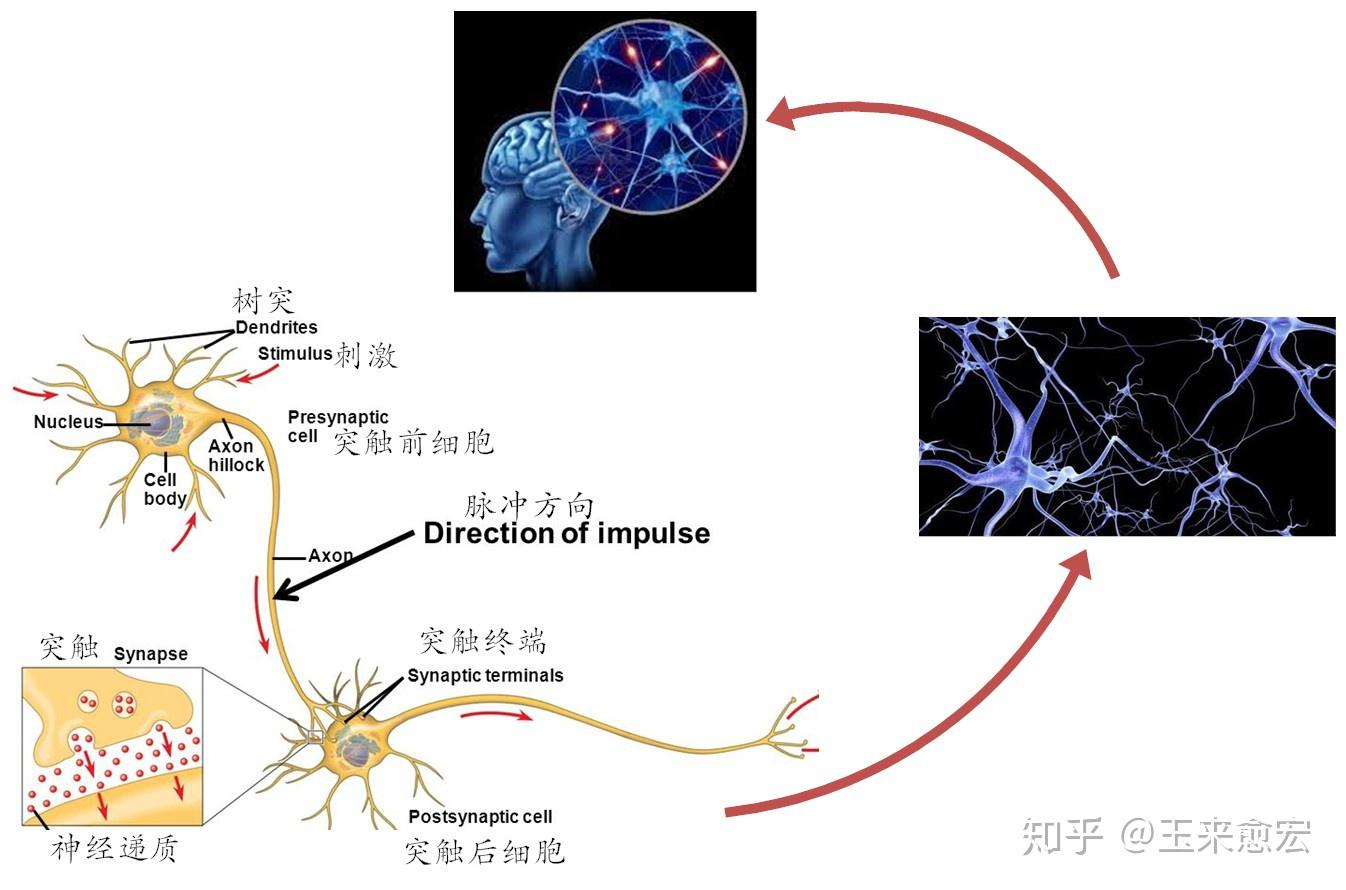
\includegraphics[width=1\textwidth]{figs/大脑神经细胞的工作流程.jpg}
\caption{大脑神经细胞的工作流程}
\label{大脑神经细胞的工作流程}
\end{figure}

\begin{figure}[htbp]
\centering
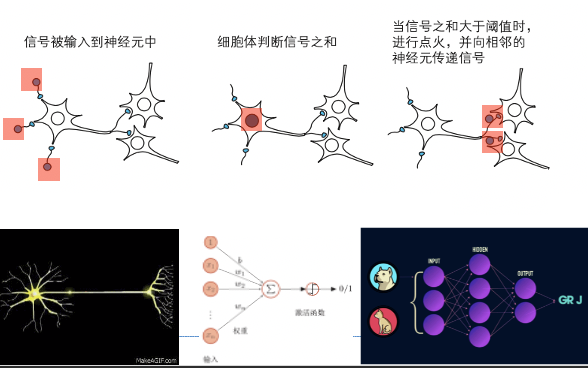
\includegraphics[width=1\textwidth]{figs/neuron.png}
\caption{生物神经元与人工神经元}
\label{生物神经元与人工神经元}
\end{figure}

具体来说，神经元的信息处理过程可分为以下五个阶段：
\begin{enumerate}
\item  {\bf 静息状态（Resting Potential）：信息存储阶段}

在未受到足够刺激时，神经元处于静息状态，%这时，细胞膜内外的钠离子（Na⁺） 和 钾离子（K⁺） 形成稳态，
细胞膜内外的电位保持稳定（约 -70mV）。这一阶段类似于一座水闸——水流虽然存在，但尚未被释放。

\item   {\bf 信号接收（Input from Dendrites）：信息采集阶段}

神经元的树突（Dendrites） 类似于雷达天线，从突触接收来自其他神经元的输入信号。输入信号可以是兴奋性（Excitatory）或抑制性（Inhibitory）信号，前者增加细胞内电位，使其更接近触发点，后者则降低电位，使其远离触发点。

\item   {\bf 动作电位触发（Action Potential Firing）：信号决策阶段}

如果输入信号的总和超过阈值（Threshold, 约 -55mV），神经元触发动作电位，形成“全或无”（All-or-Nothing）的反应——要么完全激活，要么什么都不做，类似于逻辑门（AND/OR）。
% 只有足够的输入信号才能触发“激活”。

\item  {\bf 信号传导（Propagation along the Axon）：信息高速传输阶段}

触发的动作电位沿着轴突传播，速度可达 100 m/s。
轴突通过髓鞘（Myelin Sheath） 进行加速，类似于数据传输中的光纤加速。

\item  {\bf 突触传递（Synaptic Transmission）：信息共享阶段}
信号到达轴突末端后，神经元不会直接“接触”下一个神经元，而是通过神经递质（Neurotransmitter） 进行化学信号传递。
这些化学物质穿过突触间隙（Synaptic Cleft），作用于下一个神经元的树突，引发新的信号传递。
\end{enumerate}

%\subsection{从生物神经元到人工神经网络：深度学习的启发}
\subsection{生物神经元计算模型的启示}
%（解释如何从生物神经元发展到人工神经网络，奠定人工神经网络的生物学基础）
大脑的强大计算能力源于“神经元网络、非线性激活、权重调整”等特性。虽然神经元的信号传递机制依赖于简单的电-化学反应，但其高度并行、动态可塑的连接方式使其成为迄今为止最强大的信息处理系统。人工神经网络（ANN）的设计正是受此启发，深度学习的核心概念——信息传播、非线性激活、权重调整——均可在生物神经系统中找到生物学对应。

\subsubsection*{神经元的连接与信息传播}
单个神经元的功能虽然简单，但当成千上万个神经元“抱团”工作时，它们能够完成感知、学习和推理等复杂认知任务。 
这种网络化的连接模式直接启发了人工神经网络的层级结构，即多层神经元通过权重连接，使信息逐层提取，从低级特征（如边缘、颜色）逐步抽象为高级概念（如人脸、语义）。

\subsubsection*{非线性激活：从生物神经元到深度学习}

神经元不会线性地响应所有输入，而是具有“全或无”（All-or-Nothing）特性，即只有当输入信号超过一定阈值时，才会触发神经冲动。
这一特性启发了深度学习中激活函数（Activation Function）的设计，使得人工神经网络能够学习复杂的非线性映射。

\subsubsection*{突触可塑性：权重调整的生物学基础}

生物神经系统的学习能力来源于突触可塑性（Synaptic Plasticity），即神经元之间的连接强度会随着经验不断颁布。
心理学家唐纳德·赫布（Donald Hebb） 在 1940 年代提出的赫布学习（Hebbian Learning）。是这一现象的核心原理。其核心思想可概括为：

"Fires together, wires together." —— 同时激活的神经元，其连接会变强。

突触可塑性主要表现为主要表现为长期增强（LTP） 和 长期抑制（LTD） 两种形式，即“用进废退”原则：\begin{itemize}
\item {\bf 长期增强（Long-Term Potentiation，LTP）：}—— 突触连接随着使用频率的增加而增强

频繁同时激活的神经元，其突触连接会变强，以提高未来的信息传递效率，使大脑更容易记住信息。
这类似于“熟能生巧”：使用越频繁的神经通路，传输效率越高。

在深度学习中，这类似于梯度下降调整权重，使网络收敛。

\item {\bf 长期抑制（Long-Term Depression，LTD）：} —— 突触连接随着使用减少而削弱

如果某个突触长期得不到激活，它的连接会逐渐变弱，甚至被修剪掉，大脑会“遗忘”无用的信息。
这类似于“用进废退”：不常使用的神经通路会被削弱，以优化大脑资源分配。

在深度学习中，这类似于权重衰减（Weight Decay），防止过拟合，提高泛化能力。
\end{itemize}

突触可塑性的动态调整机制，为人工神经网络的权重更新提供了生物学依据，并直接启发了误差反向传播（Backpropagation）算法的设计。

这种生物学习机制揭示了神经网络训练的基本逻辑：
\begin{center} 
学习 = 权重调整， \quad 
记忆 = 增强连接, \quad
遗忘 = 连接削弱
\end{center} 

%深度学习的核心在于“学习”，而学习的本质就是调整神经元之间的连接强度权重的调整。

神经科学的研究结果为人工神经网络的构建提供了重要启示，主要包括：

\begin{enumerate}
\item {\bf 神经元的层级结构启发了深度学习的多层神经网络}，即将简单的低层特征逐步组合成更复杂的高级特征。
\item {\bf 神经元的激活类似于非线性函数}，这促使人工神经网络引入Sigmoid、ReLU、Softmax 等激活函数。
\item {\bf 突触可塑性启发了神经网络的权重调整机制}，对应于梯度下降（Gradient Descent）和误差反向传播（Backpropagation）。
\end{enumerate}

\begin{table}[htbp]
\centering
\caption{从生物大脑到人工智能}
\begin{tabular}{|c|c|c|c|}
\hline
{\bf 特性} & {\bf  生物神经网络 } & {\bf 人工神经网络}  \\
\hline
{\bf 计算单元} &  神经元（Neuron）)  &  人工神经元（Perceptron）   \\
\hline
{\bf 连接方式}  &  突触（Synapse）& 权重（Weight） \\
\hline
{\bf 信号传递 }  &  电信号 + 化学信号 (神经递质传递) &  数值加权求和 (矩阵运算)  \\
\hline
{\bf 信号类型 }  &  脉冲式（All-or-Nothing，动作电位） &  连续值或离散值（激活函数处理）\\
\hline
{\bf 激活机制 }  &  非线性激活 &  非线性激活\\
 &  （超过阈值触发） & （ReLU、Sigmoid、Softmax 等）\\
\hline
{\bf 学习机制}  &  突触增强（LTP）或削弱（LTD）  &  误差反向传播（Backpropagation）\\
\hline
{\bf 优化方式}  & 通过经验和环境自适应调整 & 通过梯度下降优化\\
\hline
{\bf 学习时间}  & 秒、分钟、甚至数年& 毫秒到小时\\
  & （生物学习较慢但长期有效）& （训练速度快，可快速调整权重）\\
\hline
{\bf 优化方式}  & 通过经验和环境自适应调整 & 通过梯度下降优化\\
\hline
{\bf 能量效率}  & 高效，消耗极少能量 & 能耗较高\\
& 仅约 20W，大脑功耗极低） & （深度学习需要大量计算资源和电力）\\
\hline
{\bf 并行处理能力}  & 超强并行& 受限的并行性\\
 & （$10^{11}$ 个神经元并行计算）& （GPU 并行计算，但远不及大脑）\\
\hline
{\bf 信息存储方式}  & 分布式存储 & 参数存储在权重矩阵\\
& （信息存储在突触连接中） & \\
\hline
{\bf 自适应能力}  & 高度自适应，可终身学习 &  受限的适应性 \\
 & &（需大量数据训练，无法像大脑终身学习）\\
\hline
{\bf 泛化能力}  &强 & 有限\\
  &（可以举一反三，适应多种环境） & （依赖数据集，可能存在过拟合问题）\\
\hline
{\bf 容错性}  &高  & 低\\
 &（单个神经元损坏不会影响整个大脑）  & （单个权重异常可能影响整个模型）\\
\hline
{\bf 可解释性}  & 难以解释 & 部分可解释\\
& （大脑的学习机制仍未完全理解） & （可以通过梯度分析、可视化等方法理解）\\
\hline
\end{tabular}
\label{从生物大脑到人工智能}
\end{table}

表~\ref{从生物大脑到人工智能}清晰地展示了生物神经网络与人工神经网络的相似性和差异。人工神经网络作为对生物神经网络的一种数学抽象，但仍存在诸多差距，例如能耗、学习速度、适应性和泛化能力等方面。

生物大脑的学习能力为人工神经网络的构建提供了关键灵感，而深度学习的进化，在数学和计算机科学的加持下，让“智能”逐渐变得可计算、可训练、可优化。

\section{M-P模型：人工神经网络的起点 }

20 世纪 40 年代，计算机科学家开始思考如何用数学模型模拟生物神经元的行为。
1943年，神经生理学家沃伦·麦克洛克（Warren McCulloch）和数学家沃尔特·皮茨（Walter Pitts）发表了《神经活动中思想内在性的逻辑演算》（A Logical Calculus of Ideas Immanent in Nervous Activity）\cite{mcculloch1943logical}一文，被称作“神经网络天下第一文”。这篇文章中的M-P模型（McCulloch-Pitts Model）是人工神经网络的第一个数学化模型，被誉为神经网络研究的奠基之作。不仅奠定了人工神经网络的数学基础，还对计算机科学、控制论和存储程序计算机的发展产生了深远影响。

不同于弗洛伊德的心理学模型，M-P神经元模型是第一个将计算用于大脑的应用，同时也衍生出一个著名的论断

“本质上，大脑不过就是一个信息处理器。  ---计算神经学”

“M-P神经元模型”，是对生物大脑的极度简化，却成功地给我们提供了基本原理的证明。使得关于“思想”的理解，在某种程度上变得更加具有可解释性，而不必笼罩一层弗洛伊德式的神秘主义，然后在自我与本我之间牵扯不清。于是，麦克洛克曾向一群研究哲学的学生骄傲地宣布：

“在科学史上，我们首次知道了我们是怎么知道的

（For the first time in the history of science, we know how we know）。”ss

\begin{figure}[htbp] 
\centering 
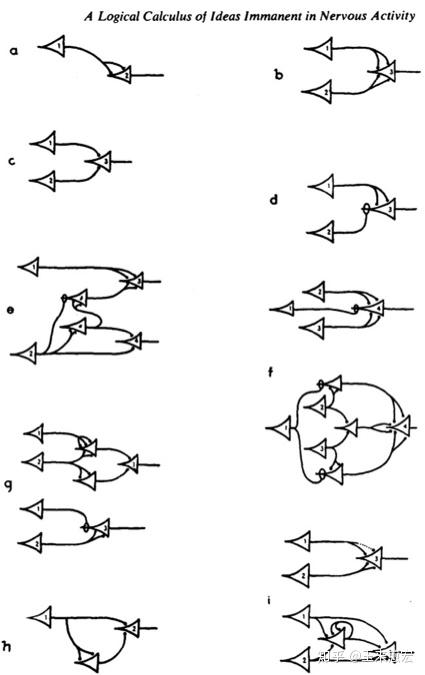
\includegraphics[width=0.6\textwidth]{figs/神经网络天下第一文《神经活动中思想内在性的逻辑演算》中的逻辑门（发表于1943年）.jpg} 
\caption{神经网络天下第一文}
\label{神经网络天下第一文} 
\end{figure}

\subsection{M-P 模型的基本结构}

M-P 模型的核心思想是，将生物神经元的工作方式简化为数学模型，用二值逻辑描述信息传递的过程。其基本计算流程如下( 如图~\ref{M-P神经元模型})：
\begin{enumerate}
\item {\bf 输入（Inputs，~$x_i$）：} 来自其他神经元的二值输入（0 或 1）。
\item {\bf 权重（Weights，~$w_i$）：}每个输入的影响程度（可以是正数或负数）
\item {\bf 加权求和（Weighted Sum, ~$S$）：}对所有输入按权重进行求和：
$$S  = \sum_{i=1}^n w_i x_i$$
\item {\bf 阈值（Threshold, ~$\theta$）：}决定神经元是否激活的临界值。
\item {\bf 激活函数（Activation Function）：}使用阶跃函数（Step Function）进行二值化：
$$
y =\left\{ \begin{array}{ll} 
1 & \mbox{ if } S\ge \theta\\
0 & \mbox{ if } S <  \theta\\ 
\end{array}\right.
$$
\end{enumerate}

 \begin{figure}[htbp]
\centering
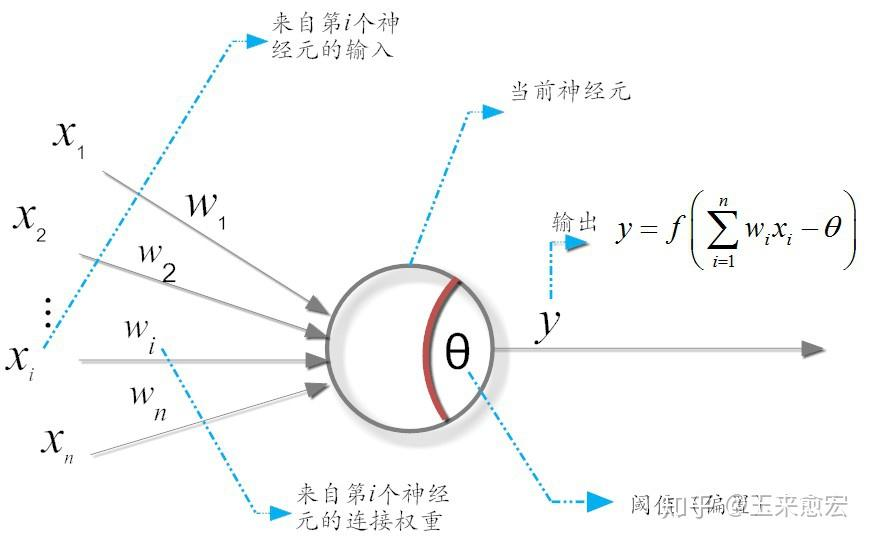
\includegraphics[width=0.8\textwidth]{figs/M-P神经元模型.jpg}
\caption{M-P神经元模型}
\label{M-P神经元模型}
\end{figure}

麦卡洛克和皮茨的神经元模型还可以被描述图~\ref{M-P模型的另一种描述}所示的样子。
\begin{figure}[htbp]
\centering
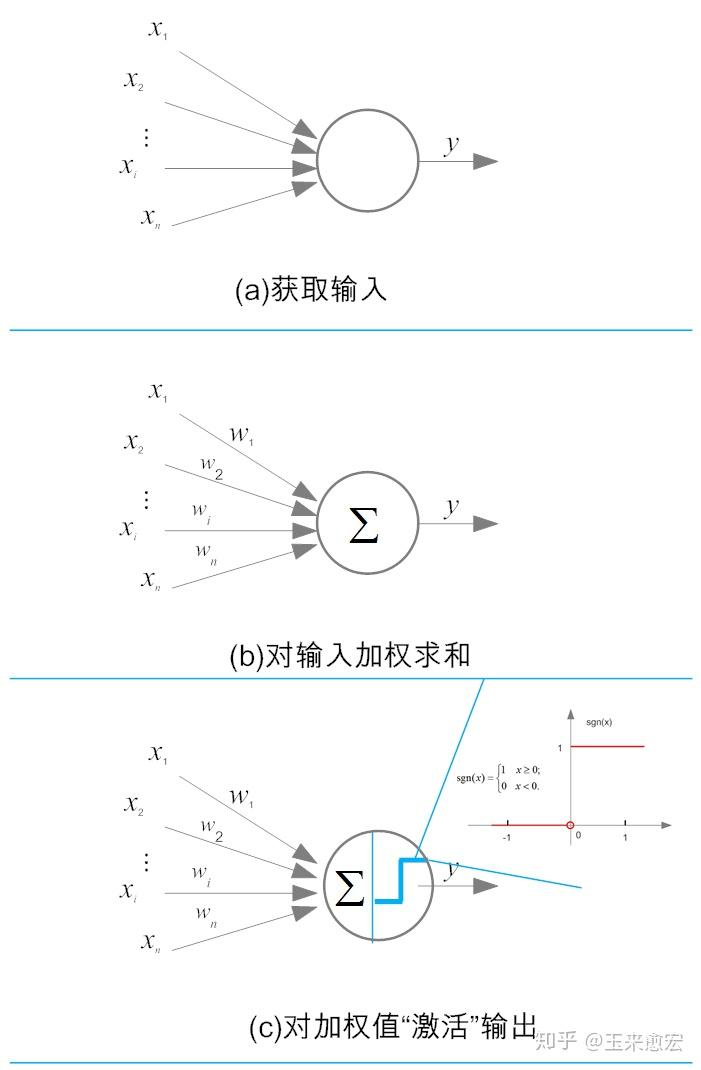
\includegraphics[width=0.8\textwidth]{figs/M-P模型的另一种描述.jpg}
\caption{M-P模型的另一种描述}
\label{M-P模型的另一种描述}
\end{figure}

图~\ref{M-P模型的另一种描述}的描述与现在神经网络中的表示几乎没什么差别了，图~\ref{M-P模型的另一种描述}(a）表示神经元从外界获得输入 ~$x_1,x_2,\dots, x_n$ (箭头模拟表示突触)，传给神经元，神经元的输出是~$y$。图~\ref{M-P模型的另一种描述}(b)突触根据不同的性质以及强度，赋予一个不同的权重，然后，神经元的输入现在升级为一个加权和。图~\ref{M-P模型的另一种描述}(c)表示的是，加权和并不是“赤裸裸”地直接输入，而是阈值函数（亦称激活函数）将“全（1）或无（0）“法则，引入到神经元结构中，这个法则模拟的是神经元激活或抑制。

M-P 神经元模型的提出，意味着我们可以把大脑视为计算机的存在，由此奠定了人工神经网络的数学基础：
\begin{itemize}
\item 神经元的状态可以用二值（0 和 1）表示：兴奋为 1，不兴奋为 0。
 \item {\bf 二值化输入和输出：} 所有输入和输出只能取 0 或 1，模拟生物神经元的“全或无”特性。
\item {\bf 神经元可以被数学化表示}——输入信号经过加权求和，并通过一个阈值函数决定是否激活输出。
\item {\bf 逻辑运算可以用神经元实现}——基本的布尔逻辑运算（如AND、OR、NOT）都可以用神经元的连接方式模拟。
%\item {\bf 神经网络具备通用计算能力}——他们证明，只要神经网络的结构足够复杂，就能够模拟任意复杂的计算任务（类似于图灵机）。
\end{itemize}

\subsection{ M-P 模型如何实现逻辑运算}

由于 M-P 模型的输出是 0 或 1，它可以直接模拟布尔逻辑运算。以下是它实现基本逻辑门的示例：

\subsubsection*{\bf 1.  AND 逻辑门}

\begin{table}[htbp]
\centering
\caption{AND 逻辑门}
\begin{tabular}{|c|c|c|c|}
\hline
{\bf $x_1$} & $x_2$ & 输出 $y$ \\
\hline
0  & 0  & 0    \\
\hline
0  & 1  & 0    \\
\hline
1  & 0  & 0    \\
\hline
1  & 1  & 1    \\
\hline
\end{tabular}
\label{AND 逻辑门}
\end{table}

设定:
\begin{itemize}
\item $w_1 =1, w_2 =1$
\item $\theta =2$ 
\end{itemize}

计算方式：
$$ S= x_1 \cdot 1  + x_2 \cdot 1$$
如果~$ S\ge 2$, 输出~$1$，否则输出~$0$。

\subsubsection*{\bf 2.  OR 逻辑门}

\begin{table}[htbp]
\centering
\caption{OR 逻辑门}
\begin{tabular}{|c|c|c|c|}
\hline
{\bf $x_1$} & $x_2$ & 输出 $y$ \\
\hline
0  & 0  & 0    \\
\hline
0  & 1  & 1   \\
\hline
1  & 0  & 1    \\
\hline
1  & 1  & 1    \\
\hline
\end{tabular}
\label{OR 逻辑门}
\end{table}

设定:
\begin{itemize}
\item $w_1 =1, w_2 =1$
\item $\theta =1$ 
\end{itemize}

\subsubsection*{\bf 3.  NOT 逻辑门}

\begin{table}[htbp]
\centering
\caption{NOT 逻辑门}
\begin{tabular}{|c|c|c|c|}
\hline
{\bf 输入$x$}  & 输出 $y$ \\
\hline
0  & 1   \\
\hline
1  & 0    \\
\hline
\end{tabular}
\label{NOT 逻辑门}
\end{table}

设定:
\begin{itemize}
\item $w =-1 $
\item $\theta =-0.5$ 
\end{itemize}

\subsubsection*{\bf 4.  异或XOR 逻辑门}

\begin{table*}[htbp]
\centering
\caption{异或XOR 逻辑门}
\begin{tabular}{|c|c|c|c|}
\hline
{\bf $x_1$} & $x_2$ & 输出 $y$ \\
\hline
0  & 0  & 0    \\
\hline
0  & 1  & 1   \\
\hline
1  & 0  & 1    \\
\hline
1  & 1  & 0   \\
\hline
\end{tabular}
\label{XOR逻辑门}
\end{table*}

设定:
\begin{itemize}
\item $\theta =-0.5$ 
\end{itemize}

M-P 模型的成功展示了简单的神经元可以通过不同的权重和阈值，实现基本的逻辑推理能力。

\subsection{M-P 模型的局限性}
尽管 M-P 模型奠定了人工神经网络的数学基础，但它存在以下主要局限性：
\begin{enumerate}
\item {\bf 无法解决非线性问题：} XOR（异或）问题无法用单个 M-P 神经元表示，因为 XOR 不是线性可分的。

\item {\bf 缺乏学习能力：}权重和阈值需要人工设定，无法通过数据训练自动优化。

\item {\bf 输入与输出的二值化限制：} M-P 模型仅支持二值输入和输出，无法表示和处理连续值或概率性信息。
\end{enumerate}

由于这些局限性，M-P 模型虽然奠定了人工神经网络的基础，但不能用于复杂的学习任务。

 M-P 模型是人工神经网络发展的第一步，它的提出不仅奠定了人工神经网络的数学基础，更在多个学科产生了深远影响。其价值主要体现在以下三个方面：
\begin{enumerate}
\item {\bf 将神经科学引入数学建模，使人工神经网络成为一个可计算的系统。 }  

M-P 模型首次将生物神经元的计算机制用数学模型描述，使神经科学与逻辑学相结合。这一突破性思路影响至今，迄今，许多研究者仍然认为，计算机智能的发展终将回归对神经科学和大脑的研究。

\item {\bf  影响计算机科学，推动存储程序计算机与控制论的发展 } 
M-P模型为现代计算机科学提供了由神经元构成的神经网络实现的逻辑计算的借鉴，另一方面，也为现代存储程序计算机的设计提供了早期理论参考，M-P模型为图灵机和现代的存储程序计算机之间，搭建了一座难以忽略的桥梁，并深刻影响了控制论、信息论的兴起。

\item {\bf  激发神经网络学习的发展，奠定深度学习的理论框架} 
M-P 模型的局限性在于无法自动学习，但它促使后续研究者不断探索如何让神经网络具备自学习能力。从皮茨开始，研究者们致力于设计可调节参数的神经网络，最终催生了 感知机（Perceptron）、多层感知机（MLP）、BP算法、卷积神经网络（CNN）、循环神经网络（RNN）、深度信念网络（DBN） 等诸多技术。它们都是致力于在不同应用场景下，自动快速找到网络的连接权值。如今，神经网络学习（包括深度学习）已经占据了人工智能领域的半壁江山，M-P模型可谓居功至伟。
\end{enumerate}

%数学化神经科学：从定性到定量的历史飞跃
M-P 模型，不仅是人工神经网络的起点，更是人类探索智能的里程碑。
从 Cajal 的神经元学说 到 麦克洛克-皮茨的数学模型之间，科学史实现了一次重要的飞跃：人类不仅能够观察神经元的行为，还能够用精确的数学语言描述和预测这些行为。

这种从定性到定量的转变，不仅使认知神经科学和脑科学脱离了玄学的边缘，更为人工智能的崛起提供了坚实的理论框架。

\begin{story}{数学天才遇上神经科学家}

麦克洛克的人生，走的是一条妥妥的精英科学家路线。他出生于美国东海岸的贵族家庭，从小接受精英教育。
在耶鲁大学研究哲学和心理学，随后在哥伦比亚大学取得心理学硕士和医学博士学位。他的研究领域横跨神经生理学、精神病学和计算理论。但麦克洛克的内心更向往哲学，希望探索知识的终极意义。%他始终想弄明白，人类的思想是否可以被数学描述？

当时，弗洛伊德的精神分析学派如日中天，而麦克洛克坚持认为，种种精神活动，包括神秘工作及精神失常，都来自于神经元的机械式反应。他更倾向于用数学和生物学解释大脑的运作方式。

相比之下，皮茨是个非典型天才——他没有上过正式大学，但他的数学才能让众多科学家惊叹。14 岁时，他便自学掌握罗素和怀特海的《数学原理》（Principia Mathematica) 靠，这是一本许多数学家都难以完全掌握的巨著。
16 岁时，他因家境贫寒流浪到芝加哥，偶然遇到了数学家鲁道夫·卡恩（Rudolf Carnap），并成为他的学生。
18 岁时，他遇到了 42 岁的麦克洛克。皮茨精通逻辑推理和计算理论，而麦克洛克正急需一个数学天才来帮助他用数学形式化描述大脑的逻辑，两人一拍即合。

两人一拍即合，皮茨的数学能力完美补足了麦克洛克的神经科学知识。

罗素等人在书中论述说，“所有的数学法则，都可自下而上地用无可辩驳的基本逻辑来建立（all of mathematics could be built from the ground up using basic, indisputable logic）”。而在底层、基础的逻辑，即为是与非两种判定。然后，通过对这两个逻辑判定进行一系列的组合操作，例如，合取（conjunction）实现“与（and）”操作、析取（disjunction）实现“或（or）”操作、取反（negation）实现“否（not）”操作，这样就可以一砖一瓦地构建起复杂的数学大厦。

受《数学原理》的启发，麦克洛克当时正尝试尝试用莱布尼茨的二进制逻辑来构建一个大脑模型。

他推测：神经元的工作机制可能类似于逻辑门电路，接受多个输入，通过阈值决定是否激活，进而执行“与”（AND）、“或”（OR）、“非”（NOT）等逻辑运算。这一思想为后来的人工神经网络奠定了理论基础。  

然而，大脑的工作方式比数学逻辑更复杂。神经元网络可能形成环状连接，即最后一个神经元的输出又成为第一个神经元的输入，这导致了逻辑悖论——“结果”成了“原因”。麦克洛克一度被这个难题困住，而皮茨巧妙地通过模数法（Modulo Mathematics）解决了这个问题，把最后一个输出巧妙地变成了第一个输入。就像时钟的数字循环一样，12 点的下一个小时不是 13，而是 1。  

从人的反应消耗能量来看，这一设置非常智能。 
神经元细胞的二元工作状态（即激发或静默），让麦克洛克联想到了莱布尼茨二进制逻辑单元以及罗素的数学构建论断。大脑的工作机制复杂而神秘，但其底层逻辑，是不是也构建于神经元的简单输出呢？

于是，麦克洛克猜想，{\bf 神经元的工作机制很可能类似于逻辑门电路，它接受多个输入，然后产生单一的输出。通过改变神经元的激发阈值以及神经元之间的连接程度，就可以让它执行“与”“或”“非”等功能。}

当时，麦克洛克刚读了一篇英国数学家阿兰·图灵（Alan Turing）的论文。
麦克洛克认为，大脑的工作机理很可能也是这样的一种机器，它用编码在神经网络里的逻辑来完成计算。如果神经元可用逻辑规则连接起来，这样就构建了结构更为复杂但功能更加强大的思维链（Chains of Thoughts）。这种方式与《数学原理》将简单命题链（Chains of Propositions）连接起来，以塑造更加复杂的数学定理，是一致的。

当麦克洛克向一群哲学学生宣布这一发现时，他骄傲地说：  “在科学史上，我们首次知道了我们是怎么知道的。”（For the first time in the history of science, we know how we know.）

他们的研究受到阿兰·图灵（Alan Turing） 的启发，尝试用逻辑演算模拟大脑的计算能力。最终，他们成功建立了M-P 神经元模型（McCulloch-Pitts Model），这是人工神经网络的第一个数学模型，开启了用数学理解智能的时代。  

几十年后，他们的思想依然影响着现代深度学习，其中的逻辑连接启发了人工神经网络，环状结构则成为了循环神经网络（Recurrent Neural Network, RNN）的重要概念。  

更多有趣内容，可以参见\cite{张玉宏2018深度学习之美}中的《牛掰扫地僧：M-P模型背后的那些人和事》。

\end{story}

\section{感知机：第一个可训练的神经网络，神经网络的“Hello World”}

感知机（Perceptrons），受启发于生物神经元，它是一切神经网络学习的起点。感知机学习，就是神经网络学习的“Hello World”，是很多从事计算机行业的人“光荣与梦想”开始的地方。

1957 年，康奈尔大学心理学教授弗兰克·罗森布拉特（Frank Rosenblatt） 在 M-P 模型基础上提出了“感知机”（Perceptron）的概念。这是第一个能够自动调整权重、进行学习的人工神经网络。  
 
所谓的感知机，其实是一个由两层神经元构成的网络结构，它在输入层接收外界的输入，通过激活函数（含阈值）的变换，把信号传送至输出层，因此它也称之为“阈值逻辑单元（threshold logic unit）”。感知机的提出标志着人工智能进入了可训练学习的阶段，因此，它被称为神经网络的“Hello World”。

感知机后来成为许多神经网络的基础，但它的理论基础依然建立于皮茨等人提出来的“M-P神经元模型”。罗森布拉特提出的感知机模型如图~\ref{罗森布拉特提出的感知机模型}所示。
\begin{figure}[htbp]
\centering
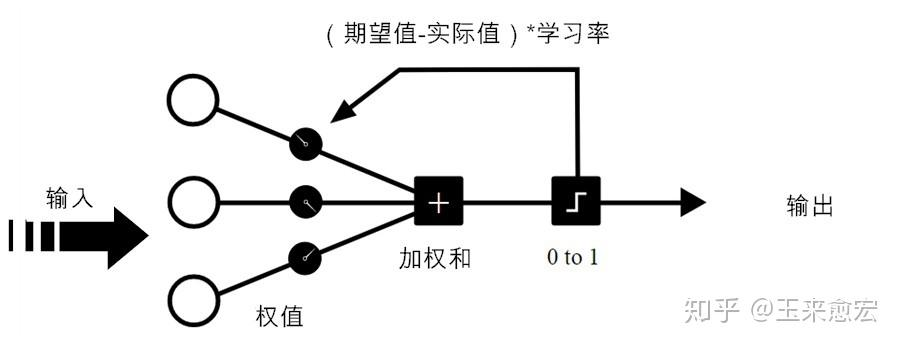
\includegraphics[width=0.8\textwidth]{figs/罗森布拉特提出的感知机模型.jpg}
\caption{罗森布拉特提出的感知机模型}
\label{罗森布拉特提出的感知机模型}
\end{figure}

对比图~\ref{M-P模型的另一种描述}和图~\ref{罗森布拉特提出的感知机模型}，感知机模型可以看作一个带有反馈机制的M-P神经元模型。

感知机虽然简单，但已初具神经网络的必备要素。在前面我们也提到，所有“有监督”的学习，在某种程度上，都是分类（classification）学习算法。而感知机就是有监督的学习，因此它也是一种分类算法。

\subsection{感知机的工作原理}
%根据感知机模型的形式化描述公式~\ref{eq:感知机}
%感知机的基本操作很简单：输入一些特征（比如颜色和形状），通过一堆加权计算，再用激活函数输出结果。如果感知机猜错了，它会调整权重，直到能准确分类。这个“试错-调整”的过程，就是机器学习的雏形。

每一次练习都是以左面的输入神经元为开端，先给每个输入神经元都赋上随机的权重，然后计算它们的加权输入之和。如果加权和为负数，则预测结果为0，否则，预测结果为1（这里的0或1，对应于图片的“左”或“右”，在本质上，感知机实现的就是一个二分类）。如果预测是正确的，则无须修正权重；如果预测有误，则用学习率（Learning Rate）乘以差错（期望值与实际值之间的差值），来对应地调整权重，如图~\ref{罗森布拉特提出的感知机模型}所示。

学着，学着，这部感知机就能“感知”出最佳的连接权值。然后，对于一个全新的图片，在没有任何人工干预的情况下，它能“独立”判定出图片标识为左还是为右。这个过程，不就与小孩子的学习差不多吗？儿童成长的第一阶段（从出生到2岁，相当于婴儿期）就是感知阶段。此阶段的儿童主要靠感觉和动作探索周围的世界，逐渐形成物体永存性观念，慢慢就有了自己对事物的独立判断。

感知机的数学表示为：
\begin{equation}\label{MLP-bias}
y = \sigma \left( \sum_{i=1}^n w_i x_i +b\right)
\end{equation}
其中，~$w_i$ 为权重，~$x_i$为输入信号，~$\theta$ 为偏置，~$\sigma$ 为激活函数（如阶跃函数）。
除了神经元的权重连接之外，神经元内部还有一个施加于自身的特殊权值---偏置（bias），即\eqref{MLP-bias}中的~$\theta$。偏置决定了神经元的连接加权和得有多大，才能让激发变得有意义。

感知机的目标是通过训练学习输入和输出之间的映射关系。它采用简单的更新规则优化权重：
 $$ w_i \leftarrow w_i+ \eta ( y_{\rm target}- y_{\rm actual}) x_i$$
 其中，~$x_i$为输入，~$\eta$为学习率，~$ y_{\rm target}$为期望的真实输出，~$ y_{\rm actual}$为模型的当前输出值。 

具体地，感知机的运行包括以下三个步骤：

\begin{enumerate}
\item {\bf 输入数据加权求和：}

每个输入~$x_i$ 乘以相应的权重~$w_i$，然后求和
 \begin{equation*} 
S = \sum_{i=1}^n  w_i x_i - \theta
\end{equation*}
其中~$\theta $ 是阈值。
非齐次项$-\theta$通常用~$b$ 表示并被称作偏置(bias）。于是有
 \begin{equation}\label{eq:感知机决策函数} 
S = \sum_{i=1}^n  w_i x_i + b
\end{equation}
\item {\bf 通过激活函数决定输出类别：} 

计算的结果~$S$ 通过阶跃函数（step function）处理：
\begin{equation}\label{eq:感知机输出}
y = {\rm sgn}(S) = \left\{ \begin{array}{ll} 
1 & \mbox{ if } S\ge 0\\
0 & \mbox{ if } S < 0\\ 
\end{array}\right.
\end{equation}
这样，感知机实现了一个二分类任务。

\item {\bf 使用误差反馈训练（感知机学习规则）：}
%使用感知机学习规则调整权重，使得模型能够适应新的数据。

如果预测（分类）错误，则触发学习规则。我们应用如下的感知机权重更新规则：
\begin{eqnarray}\label{eq:感知机-权重更新}
w_i  \leftarrow w_i +\eta ( y_{\rm target}- y_{\rm actual} )x_i,  \\ \
  \theta \leftarrow \theta + \eta  ( y_{\rm target}- y_{\rm actual} ) \times 1 = \theta + \eta  ( y_{\rm target}- y_{\rm actual} ) 
\end{eqnarray}
其中~$\eta$ 是学习率，$ y_{\rm target}$ 为期望输出的真实值，$ y_{\rm actual}$ 为感知机的当前输出值。

不断迭代，直到感知机能够在给定的训练集上实现正确分类。 

预测“误差”就是整个网络中权值和阈值的调整动力。“知错能改，善莫大焉。”
很显然，如果为0，即没有误差可言，那么新、旧权值和阈值都是一样的，网络就稳定可用了。

感知机参数学习的更新过程
感知机的负反馈纠偏机制

\end{enumerate}

\begin{figure}[htbp]
\centering
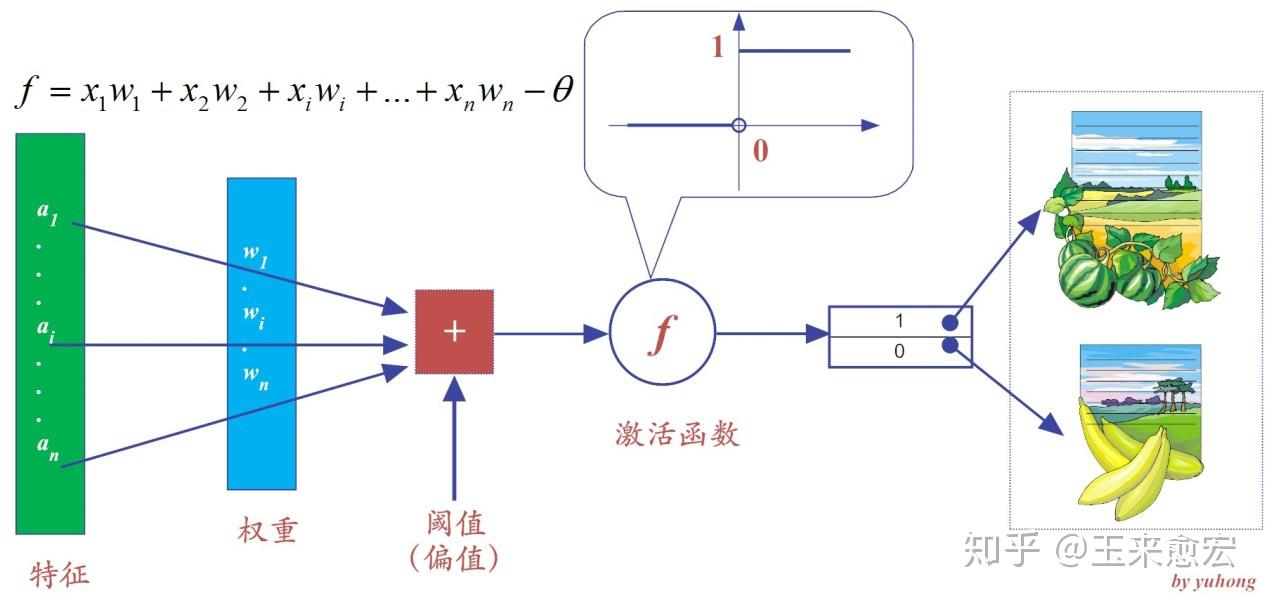
\includegraphics[width=0.8\textwidth]{figs/感知机学习算法示意图.jpg}
\caption{感知机学习算法示意图}
\label{感知机学习算法示意图}
\end{figure}

%\begin{figure}[htbp]
%\centering
%\begin{subfigure}{0.9\linewidth}
%\centering
%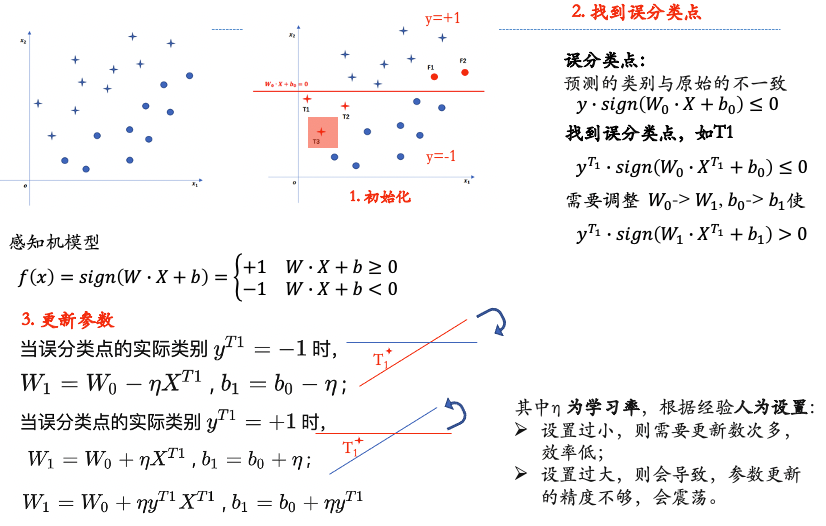
\includegraphics[width=1\linewidth]{figs/参数更新1.png}
%\caption{参数更新过程一}
%\label{参数更新1}
%\end{subfigure}
%
%\begin{subfigure}{0.9\linewidth}
%\centering
%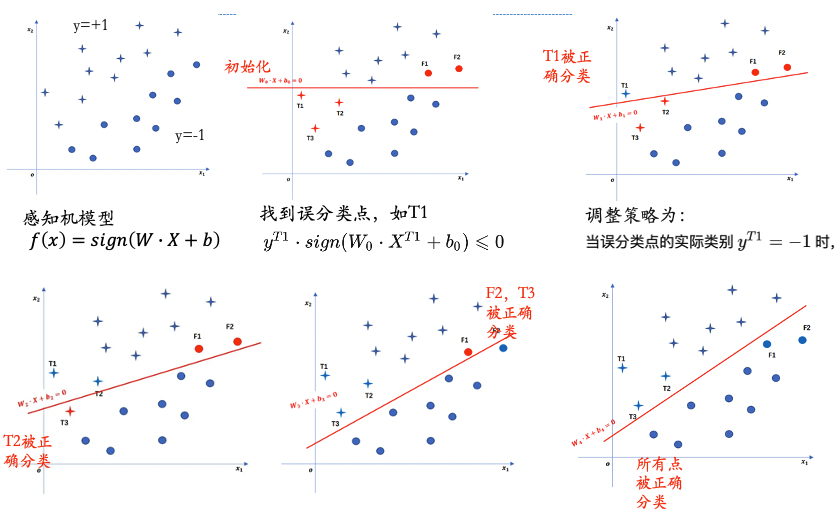
\includegraphics[width=1\textwidth]{figs/参数更新2.png}
%\caption{生物神经元与人工神经元}
%\label{参数更新2}
%\end{subfigure}
%\caption{参数更新过程一}
%\label{感知机参数学习的更新过程}
%\end{figure}

放到机器学习领域，这句话显然属于“监督学习”的范畴。因为“知错”，就表明事先已有了事物的评判标准，如果你的行为不符合（或说偏离）这些标准，那么就要根据“偏离的程度”，来“改善”自己的行为。

下面，我们就根据这个思想来制订感知机的学习规则。

从前面的讨论中，我们已经知道，感知机学习属于“有监督学习”（即分类算法）。感知机有明确的结果导向性。

这有点类似于“不管白猫黑猫，抓住老鼠就是好猫”的说法，不管是什么样的学习规则，能达到良好的分类目的，就是好的学习规则。

我们知道，对象本身的特征值，一旦训练样本确定下来就不会变化，可视为常数。

因此，所谓的神经网络的学习规则，就是调整神经元之间的连接权值和神经元内部阈值的规则（这个结论对于深度学习而言，依然是适用的）。

\subsection{感知机示例：“西瓜 vs 香蕉”分类}

在本节中，我们列举一个区分“西瓜和香蕉”的经典案例，来看看如何训练感知机，使其能够区分西瓜和香蕉。 

为了简单起见，假定西瓜和香蕉都仅有基于视觉刺激最容易得到的两个特征（feature）：颜色(绿色或黄色) 和形状(圆形和弯形)，其它特征暂不考虑。
设特征~$x_1$取值为1若颜色为绿色，反之取值为-1若颜色为黄色；同样，特征~$x_2$取值为1若形状为圆形，反之取值为-1若形状为弯曲状。 特征的取值如表~\ref{西瓜与香蕉的特征值表}所示。

假设感知机的输出数字化，如果输出为“1”则代表分类为“西瓜”，而输出为“0”代表分类为“香蕉”。
假设初始权重为~$w_1 =1, w_2 =-1, b =1$。

接下来，我们根据感知机的参数更新流程逐步获得能将西瓜和香蕉分类正确的感知机。

\begin{table}[htbp]
\centering
\caption{西瓜与香蕉的特征值表}
\begin{tabular}{|c|c|c|c|
}
\hline
{\bf 品类} & {\bf  颜色($x_1$) } & {\bf 形状($x_2$)}  \\
\hline
{\bf 西瓜} &  1 (绿色)  &  1 (圆形)   \\
\hline
{\bf 香蕉}  &  -1 (黄色) & -1 (弯形)  \\
\hline
\end{tabular}
\label{西瓜与香蕉的特征值表}
\end{table}

%，其结果分别如图\ref{感知机的输出}(a)所示：
%
%\begin{figure}[htbp]
%\centering
%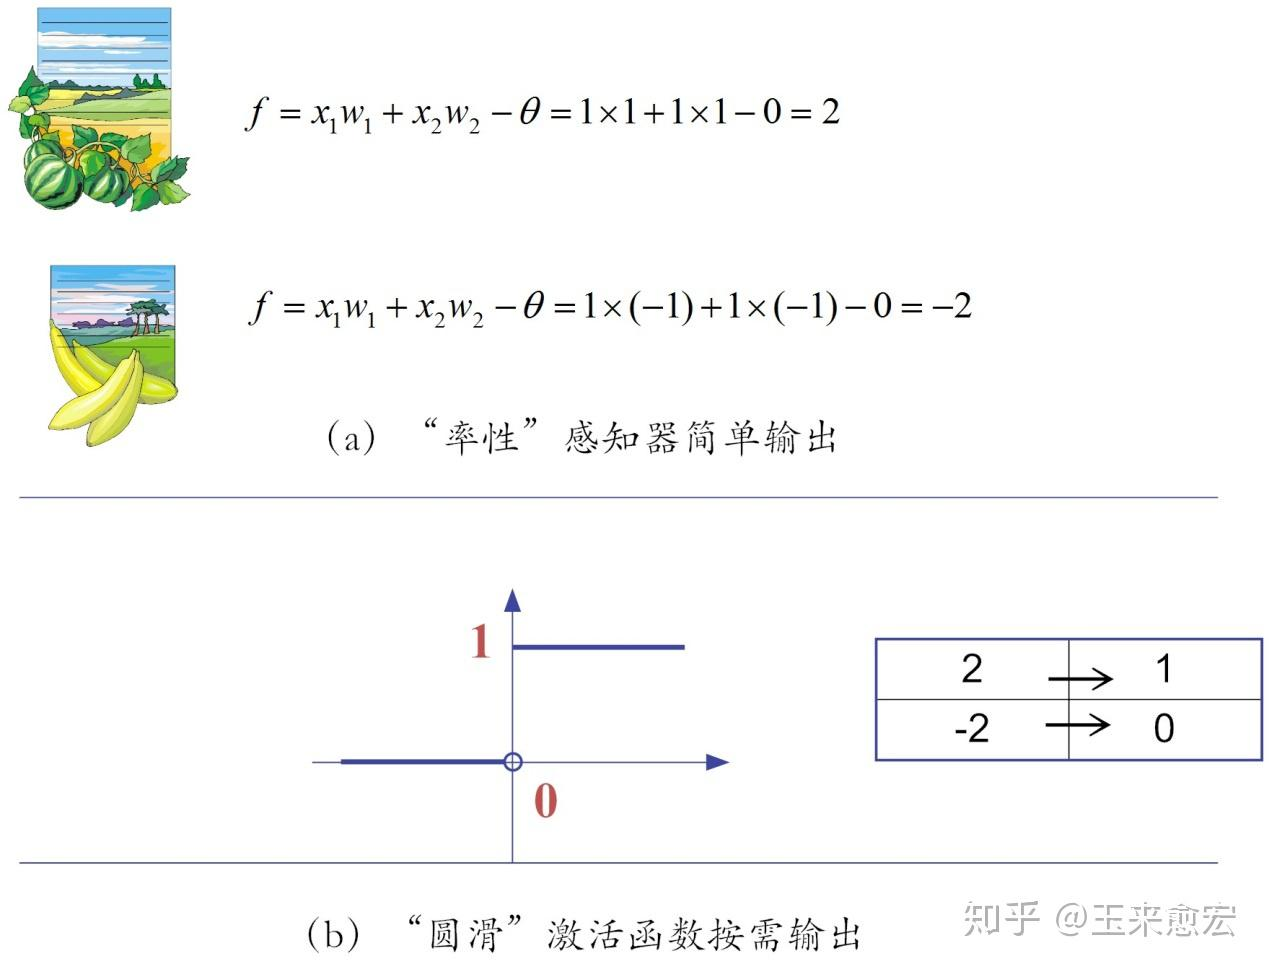
\includegraphics[width=0.8\textwidth]{figs/感知机的输出.jpg}
%\caption{感知机的输出}
%\label{感知机的输出}
%\end{figure}
 
 %下面，我们就用上面的学习规则来模拟感知机的学习过程。假设w1和w2的初始值随机分配为1和-1（注意，已经不再是前面提到的1和1了！），阈值依然为0（事实上为其他初值也是可行的，这里仅为说明问题而做了简化），那么我们遵循如下步骤，即可完成判定西瓜的学习。

 （1）计算西瓜的分类。对于西瓜，特征~$x_1 =x_2=1$。于是决策函数
$$
S  = w_1 x_1 +w_2 x_2  +b   = 1\times 1 + (-1)\times 1 + 1 = 1 >0
$$
根据公式~\eqref{eq:感知机输出} ，输出~$y_{\rm actual}=1$，即感知机实际输出“西瓜”，分类正确。

同样，计算香蕉的分类。对于香蕉，特征~$x_1 =x_2=-1$。于是决策函数
$$
S  = w_1 x_1 +w_2 x_2  +b   = 1\times (-1) + (-1)\times (-1) + 1 = 1 >0
$$
根据公式~\eqref{eq:感知机输出} ，输出~$y_{\rm actual}=1$，即感知机实际输出“西瓜”，分类错误。

（2）计算预测误差：
$$ \epsilon = y_{\rm target}- y_{\rm actual}  =0 -1=-1 $$

（3）由于香蕉的分类错误，需要纠偏。而纠偏，就需要利用公式~\eqref{eq:感知机-权重更新}所示的学习规则更新网络的权重和阈值：
$$\begin{array}{l}
 w_i  \leftarrow w_i +\eta \epsilon x_i, \quad  i=1,2, \\
  b = b+\eta \epsilon .
\end{array}
$$
为了简化计算，假设学习率~$\eta =1$。于是， 
\begin{eqnarray*}
w_1  \leftarrow w_1 +1\times (-1)\times  (-1) = 1 +1 =2, \\
w_2  \leftarrow w_2 +1\times (-1) \times   (-1) = -1+ 1 = 0, \\
b  \leftarrow 1+1 \times (-1) = 0
\end{eqnarray*}

在新一轮的网络参数（即权值、阈值）重新学习后，我们再次输入香蕉的属性值，测试一下，看看它能否正确判定：
$$ S =w_1  x_1 + w_2  x_2 +b = 2\times  (-1) + 0\times  (-1)   +0 = -2$$
再经过激活函数（阶跃函数）处理后，实际输出结果~$y_{\rm actual}=0$，分类为香蕉，预测正确！

我们知道，一个对象的类别判定正确，不能算好。于是，在判定香蕉正确后，我们还要尝试在这样的网络参数下，看看西瓜的判定是否正确的。对于西瓜，~$x_1 =x_2 =1 $，于是决策函数
$$ S =  w_1 x_1 +  w_2 x_2  +b = 2 \times 1 +0\times 1 +0   = 2$$
类似的，经过激活函数（阶跃函数）处理后，实际输出结果$y_{\rm actual}=1$，分类为西瓜，判定正确。

在这个示例里，仅仅经过一轮“试错法”（Try-Error），感知机学会了如何区分西瓜和香蕉。 但这是一个“Hello World”版本的神经网络呢！事实上，在有监督的学习规则中，我们需要根据输出与期望值的“落差”，经过多轮重试，反复调整神经网络的权值，直至这个“落差”收敛到能够忍受的范围之内，训练才告结束(示意图~\ref{感知机学习算法示意图})。这里的“试错”其实就是感知机的学习过程。

\subsection{感知机算法的直观理解}
感知机的学习过程可以看作一个“自我修正”过程，其调整方向由误差 $ y_{\rm target} - y_{\rm  actual}​$ 确定，而调整幅度则取决于输入特征~$x_i$，特征值较大者调整幅度也更大。具体的权重调整规则如下：
\begin{itemize}
\item 如果分类正确，则无需调整；
\item 如果分类错误，则根据误差进行调整：
\begin{itemize}
\item 若样本应判定为 1，但误判为 0，则增加相关特征的权重，使其更倾向于 1 。
\item 若样本应判定为 0，但误判为 1，则减少相关特征的权重，使其更倾向于 0。
\end{itemize}
\end{itemize}
这种误差反馈机制，使得感知机能够逐步优化自身的分类能力，最终找到合适的决策边界。

感知机虽然是一个简单的神经网络模型，但提出了几个关键概念：
\begin{enumerate}
\item {\bf 可学习权重}
相较于 M-P 模型的固定权重，感知机能够通过数据训练自动调整权重，从而具备了“学习”能力。

\item {\bf  误差反馈训练} 
通过感知机学习规则（Perceptron Learning Rule），感知机可以根据分类错误调整权重，改进分类能力。这一机制成为现代神经网络梯度下降算法的早期雏形。
\item {\bf 误差反馈训练：} 感知机学习规则（Perceptron Learning Rule）使其能利用分类误差调整权重，这一机制成为现代神经网络梯度下降算法的早期雏形。
\end{enumerate}

\subsection{感知机的几何意义}
数学上，感知机的决策边界实际上是一个超平面：
$$
S  = w_1 x_1 +w_2 x_2  + \cdots + w_n x_n + b   =  0
$$
这一超平面将数据空间划分为两个区域：超平面一侧的数据点被分类为 1，而另一侧的数据点被分类为 0。

在二维空间中，超平面是一条直线，而在 三维空间，它是一个平面，在更高维度（如 100 维或 1000 维）中，超平面难以直观可视化。

在训练过程中，感知机不断调整超平面的位置和方向，直到所有训练数据都被正确分类。
具体地，对每个误分类的样本，调整权重，使其朝向正确分类方向移动，其中调整偏置 $b$ 相当于平移决策边界。如果数据是线性可分的，如果数据是线性可分的，感知机算法会在有限步内收敛，最终找到一个能够正确分类所有样本的超平面。

\begin{figure}[htbp]
\centering
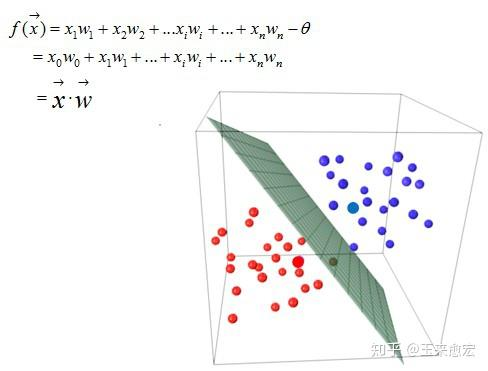
\includegraphics[width=1\textwidth]{figs/感知机的超平面.jpg}
\caption{感知机的超平面}
\label{感知机的超平面}
\end{figure}

\subsection{感知机的局限性：XOR 问题与神经网络的停滞}
尽管感知机的提出标志着人工神经网络的初步形成，但它存在一个重大局限性：无法解决线性不可分问题（如 XOR）。感知机能够完美解决线性可分问题（如 AND 和 OR），因为它们的决策边界可以用一条直线分割，但，其决策边界是非线性的，如图所示：

\begin{equation} \label{XOR}
\mbox{ XOR (异或) 逻辑：} 
\left\{ 
\begin{array}{c}
0 \oplus 0=0 \\
0 \oplus  1=1 \\
1 \oplus 0=1 \\
1\oplus  1=0 \\
\end{array}
\right.
​\end{equation} 
XOR（异或）的数据分布无法用一条直线分开，因此单层感知机无法拟合这种逻辑关系。

1969 年，马文·明斯基（Marvin Minsky） 和 西摩·帕珀特（Seymour Papert） 在《感知机（Perceptrons）》\cite{marvin1969perceptrons}一书中指出：

“单层感知机无法学习 XOR 逻辑，因为 XOR 是线性不可分的，而感知机仅能处理线性可分数据。”

由于当时尚未找到有效的解决方法，这一发现对神经网络的研究造成了沉重打击，直接导致了1970-1980 年代神经网络研究的停滞。
直到 1980 年代，多层神经网络（MLP） 和 反向传播算法（Backpropagation） 的提出，才打破了这一局限。
感知机的局限性催生了多层神经网络（MLP）的发展，推动了更复杂神经网络的研究。 

\subsection{ 感知机的实际应用}
尽管感知机是一个相对简单的神经网络模型，但它仍然可以用于一些基础的分类任务，如：

应用1：图像分类

感知机可以用于简单的二分类任务，如判断一张图片是“猫”还是“狗”。

\begin{figure}[htbp]
\centering
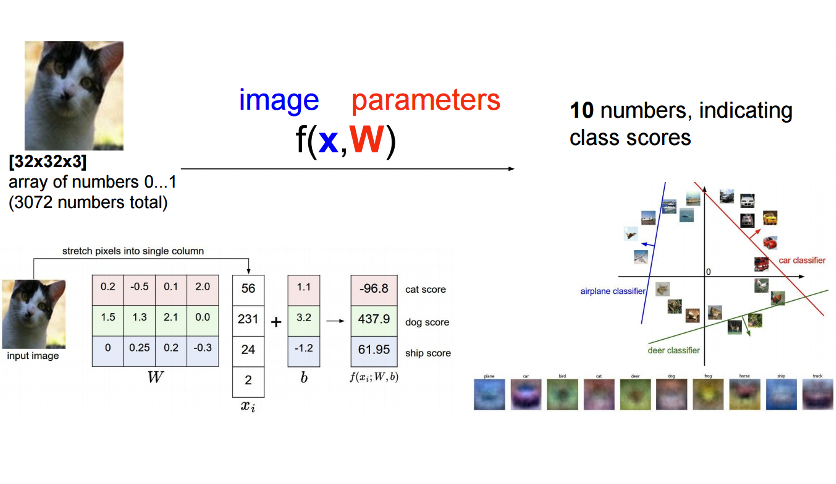
\includegraphics[width=1\textwidth]{figs/图像分类.png}
\caption{图像分类}
\label{图像分类}
\end{figure}

应用2：文本分类

在自然语言处理（NLP）中，感知机可用于垃圾邮件分类或情感分析。例如，输入邮件内容中的关键词（如“免费”“中奖”“折扣”等），可以判定是否为垃圾邮件。

\begin{figure}[htbp]
\centering
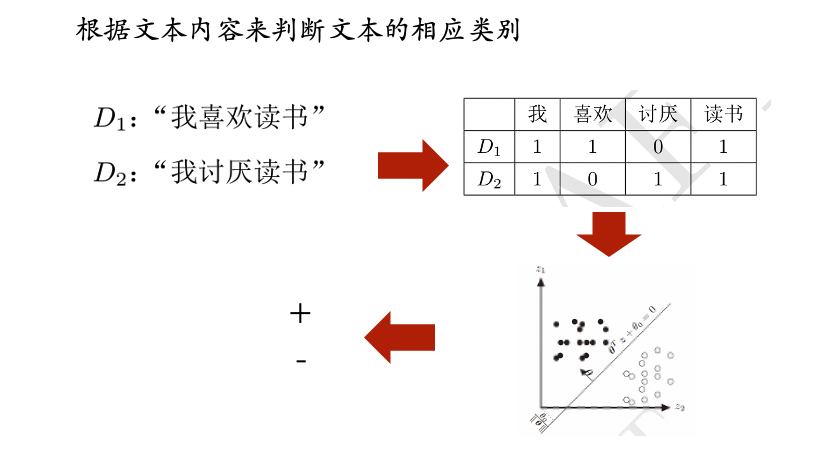
\includegraphics[width=1\textwidth]{figs/文本分类.png}
\caption{文本分类}
\label{文本分类}
\end{figure}

\subsection{ 感知机的历史影响}
感知机的提出不仅是人工神经网络的开端，更是机器学习迈向自主学习的第一步。

在人工神经网络领域中，感知机也被指为单层的人工神经网络，以区别于更复杂的多层感知机（Multilayer Perceptron, MLP）。 

作为最简单的前馈神经网络，感知机虽然结构简单，但它首次实现了参数自动更新，使机器具备了“学习”能力。这一突破使其能够通过训练调整权重，解决一定复杂度的分类问题。

感知机的另一个重大贡献是误差反馈机制，它提出了基于分类误差调整权重的学习规则，为后来的梯度下降（Gradient Descent）等优化算法提供了启发。这一机制使得机器不仅能执行计算，还能根据错误不断优化自身，为现代深度学习奠定了重要基础。

然而，感知机的线性分类特性限制了其能力，使其无法处理非线性可分问题（如异或 XOR问题）。这一缺陷导致单层感知机逐渐被更强大的多层神经网络（MLP） 所取代。然而，感知机仍然是人工神经网络演化的起点，其核心思想催生了更强大的深度学习技术，并影响了现代人工智能的发展。后续神经网络的发展奠定了坚实的理论基础。

更多细节，请参见 （第12章：感知机是如何工作的？， \cite{张玉宏2018深度学习之美}）

\begin{story}{感知机的传奇人物：弗兰克·罗森布拉特} 
弗兰克·罗森布拉特（Frank Rosenblatt） 不仅是一位杰出的科学家，更是一位充满探索精神的“折腾王”。白天他在实验室研究蝙蝠的大脑，夜晚则在自家后山搭建天文台，试图与外星生命交流。他的研究跨越神经科学、心理学和计算机科学，为智能学习理论奠定了基础。

1949年，唐纳德•赫布（Donald Hebb，1904—1985）在《行为的组织》一书中，提出了{\bf 神经心理学理论}，认为{\bf 神经网络的学习过程发生在神经元之间的突触部位，突触的连接强度会随着突触前后神经元的活动而变化，变化的幅度与两个神经元之间的活性和成正比}。这一假说为人工神经网络的发展提供了生物学依据。

受到赫布假说的启发，1958年，30岁的罗森布拉特提出了感知机（Perceptron），在工程上模拟实现了赫布假说。这是第一种能够自我学习的人工神经网络。在罗森布拉特的实验中，感知机能够学习识别50 组图片的左右方向，这是机器视觉和模式识别的早期尝试。这一突破立即引发了学术界和媒体的广泛关注。

1958 年 7 月 8 日，《纽约时报》在头版刊登了关于感知机的报道，称其为：
{\bf“ 一个能够行走、拥有视觉、能够写作、能自我复制，且有自我意识的电子计算机的雏形”。}

当时，距离标志着人工智能学科诞生的达特茅斯（Dartmouth）会议，仅仅过去两年，人工智能仍处于萌芽阶段。然而，媒体的热情远远超出了学术界的预期，《纽约时报》非常乐观地估计，
“再花上10万美元，一年以后，上述构想就能实现可期。那时，机器能够识别人类，还能把人们演讲的内容即时地翻译成另一种语言或记录下来。”
这在当时看似天方夜谭，但六十多年后的今天，这些愿景几乎都已成真。

罗森布拉特本人也信心满满，几天后，他亲自撰写了一篇文章——《Electronic 'Brain' Teaches Itself》（能自学的电脑），进一步向公众介绍他的研究。他表示：

“感知机将成为第一个能够感知、识别、适应环境的非生命智能体。”

在某种程度上，我们如今所熟知的“计算机（Computer）”一词在人工智能语境下的广泛传播，或许也与他的宣传密切相关。

尽管感知机本身存在诸多局限性，例如无法解决线性不可分问题（如 XOR 问题），但它开启了机器学习自主学习的可能性，并催生了多层感知机（MLP）和深度学习的发展。

科技预言家凯文·凯利（Kevin Kelly）在《必然》中提出，未来科技的 12 大进化趋势之一是“知化（Cognifying）”——让一切事物具备认知能力。
凯文•凯利认为，人工智能的本质就是“知化”，即硬件问题软件化。
回看罗森布拉特的感知机，正是“知化”理念的雏形。虽然感知机并未直接实现《纽约时报》所预言的所有功能，但它确实点燃了人类对智能机器的期待。六十多年后的今天，计算机视觉、语音识别、自动翻译、智能写作早已成为现实，而神经网络，正是这些技术背后的核心支撑。

罗森布拉特的大胆畅想，放在今天来看，依然不过时。
\end{story}

\section{ 多层感知机（1980s 复兴）：突破单层感知机的局限}
\subsection{增加隐藏层：解决线性不可分问题}

尽管感知机的提出奠定了神经网络的基础，但其最大局限在于无法解决线性不可分问题，例如 XOR（异或）问题。

研究者们发现，单层感知机只能学习线性可分数据，要解决 XOR 这样的非线性问题，必须在输入层与输出层之间增加隐藏层（Hidden Layer），提升网络的表达能力。这一改进催生了{\bf 多层感知机（MLP, Multilayer Perceptron）}，即深度神经网络的前身。
1974年，Geoffrey Hinton提出“多则不同”---将多个感知机连接成一个分层网络，从而可处理非线性可分问题。

MLP 的结构：
\begin{itemize}
\item {\bf  输入层：}接收数据并传递给网络
\item {\bf  隐藏层：}逐层提取数据中的复杂特征
\item {\bf  输出层：}根据学习到的特征进行最终分类
\end{itemize}

\begin{figure}[htbp]
\centering
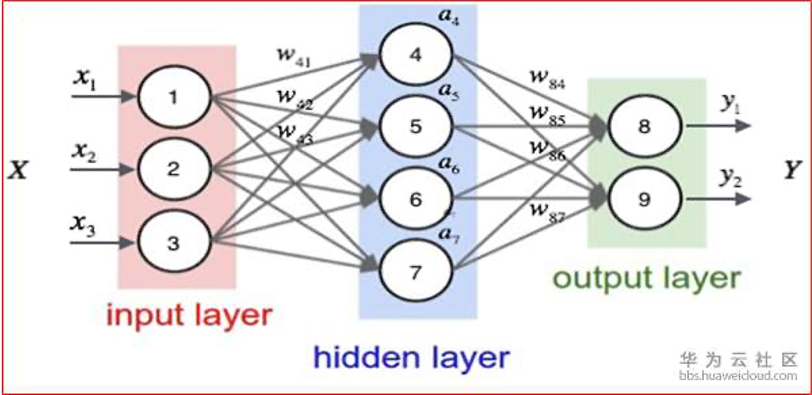
\includegraphics[width=0.8\textwidth]{figs/MLP.png}
\caption{多层感知机网络}
\label{MLP}
\end{figure}
  
\subsection{两层感知机如何解决“异或”问题}
多层感知机（MLP）之所以能够解决 XOR（异或）问题，关键在于隐藏层的引入。
以下是一个两层感知机（输入层 + 隐藏层 + 输出层）实现 XOR 的示例。%，如图~\ref{可解决“异或”问题的两层感知机}所示。

对于 XOR 逻辑~\ref{XOR}
\begin{figure}[htbp]
\centering
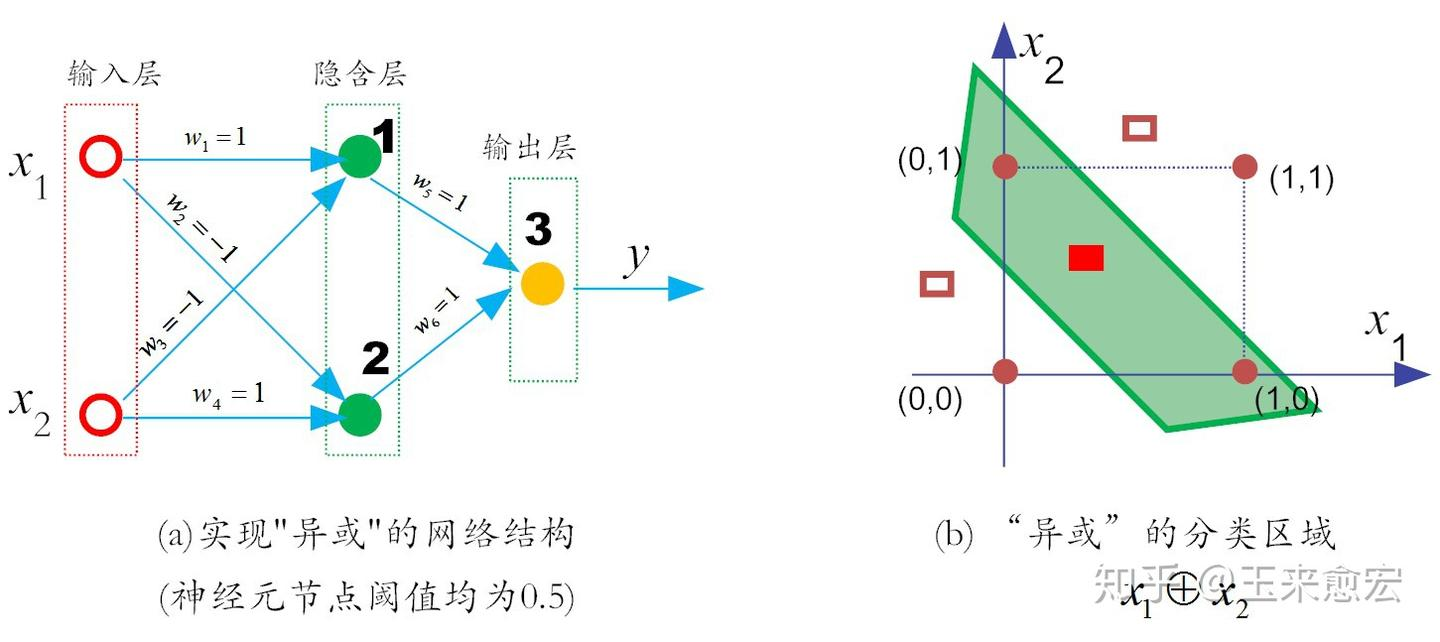
\includegraphics[width=1\textwidth]{figs/可解决“异或”问题的两层感知机.jpg}
\caption{可解决“异或”问题的两层感知机}
\label{fig:可解决“异或”问题的两层感知机}
\end{figure}

假设在如图~\ref{fig:可解决“异或”问题的两层感知机}所示的神经元（即实心圆），其激活函数依然是阶跃函数（即{\rm sgn}函数），它的输出规则非常简单：当~$x\ge 0$ 时，~$f(x)$输出为1，否则输出0。

假设神经元~$x_1$对隐藏层节点1和2的权重分别为~$w_1=1$和~$w_2=-1$，且神经元~$x_2$对隐藏层的节点1和2的权重分别为$w_3=-1$和$w_4=1$，偏置~$b =-0.5$。

假设神经元~$x_1$ 和~$x_2$ 具有相同的输入，例如 $x_1= x_2=1$。此时，隐藏层的神经元1的输出为：
$$
f_1 =w_1 x_1 +w_2x_2 +b =  {\rm sgn}\left( 1 \cdot 1 + 1\cdot (-1) -0.5 \right) =  {\rm sgn}(-0.5) =0.
$$
类似地，对于隐藏层的神经元2，有
$$
f_2 = w_1 x_1 +w_2x_2 +b = {\rm sgn}\left( 1 \cdot (-1) + 1\cdot 1 -0.5\right) =  {\rm sgn}(-0.5) =0.
$$

现在到了输出层，对于输出神经元3而言，这时~$f_1$和~$f_2$是它的输入，于是有：
$$
y = f_3 =w_1 f_1 +w_2f_2 +b =  {\rm sgn}\left( 0 \cdot 1 + 0\cdot (-1) -0.5\right) =  {\rm sgn}(-0.5) =0.
$$
因此，当~$x_1$和~$x_2$同为1时，神经网络输出~$0$。

同理，可以验证，当神经元~$x_1$和~$x_2$的输入同为~$0$时的情况，这个简单的两层感知机输出为~$0$。

现在假设神经元~$x_1$和~$x_2$的输入不相同，不妨设~$x_1=1$而~$x_2=0$。因此，对于隐藏层的神经元1，有
$$
f_1 ={\rm sgn}(w_1x_1 + w_2x_2 +b) ={\rm sgn}(1\times 1 +(-1)\times 0-0.5) ={\rm sgn}(0.5) =1,
$$
而对于隐藏层的神经元2，有
$$
f_2 ={\rm sgn}(w_3x_1 + w_4x_2 +b) ={\rm sgn}( (-1)\times1 +1\times 0-0.5) ={\rm sgn}(-1.5) =0
$$
然后，对于输出层的输出神经元3而言，这时~$f_1$和~$f_2$是它的输入，于是有：
$$
y=f_3 ={\rm sgn}(w_5f_1 + w_6f_2 +b) ={\rm sgn}(1\times 1 +0\times 0-0.5) ={\rm sgn}(0.5) =1
$$

不失一般性，由于~$x_1$和~$x_2$的地位是可以互换的。因此有，当~$x_1$和~$x_2$取值不同时，感知机输出为1。

由上面的分析可知，如图~\ref{fig:可解决“异或”问题的两层感知机}所示的两层感知机实现了“异或”功能。

需要说明的是，能够完成“异或”功能的网络权重也不是唯一的。以上神经网络中的权值和阈值是我们事先给定的，而实际上，它们是需要神经网络自己通过反复地“试错”学习而来。

如前文所述，想解决“异或”问题，就需要让网络复杂起来。这是因为，复杂的网络，表征能力就比较强。按照这个思路，可以在输入层和输出层之间，添加一层神经元，将其称之为隐含层（hidden layer，亦有文献简称为“隐藏层”、“隐层”，后文不再区分这三个称谓）。

\subsection{真正的突破：反向传播（Backpropagation）}
虽然多层感知机（MLP）的结构在 1970 年代已被提出，但如何高效地训练多层感知机仍然是一个难题。
由于 MLP 采用隐藏层，误差不像单层感知机那样可以直接计算和修正。%，而是需要一种机制，将误差从输出层逆向传递到隐藏层，使整个网络能够逐层调整权重。

这一难题直到 1986 年 才被突破，杰弗里·辛顿（Geoffrey Hinton）等人提出了反向传播算法（Backpropagation, BP），通过梯度下降来优化权重，使多层神经网络的训练成为可能。

反向传播（BP） 的本质是通过 梯度下降（Gradient Descent） 来优化神经网络的权重，使网络的输出误差逐步减小。

其核心步骤包括：
\begin{enumerate}
\item {\bf 前向传播（Forward Propagation）} 

输入数据经过网络，依次通过输入层 → 隐藏层 → 输出层，得到预测值 $ \hat{y} $。

\item {\bf 计算输出误差（Loss Computation）}

计算预测值 $ \hat{y} $ 与真实值 $ y $ 之间的误差。常用的误差函数（损失函数）包括
$$ \mbox{均方误差（MSE）：}  L= \frac{1}{2}\left( y-\hat y \right)^2 
$$
和
$$ \mbox{交叉熵损失（Cross Entropy Loss）：}  L= -\sum y_i {\rm log} \hat y_i
$$
\item {\bf 误差反向传播（Backward Propagation）}

误差从输出层向隐藏层反向传播，通过链式法则（Chain Rule） 计算各层的梯度：
$$ \frac{\partial L}{\partial w} =\frac{\partial L}{\partial \hat y}\cdot \frac{\partial \hat y}{\partial w}  $$
这一过程涉及 梯度计算，确保误差能够层层传递。
\item {\bf 更新权重（Weight Update）}
采用 梯度下降法（Gradient Descent），调整网络参数：
$$  
w^{(t+1)}= w^{(t)} -\eta  \frac{\partial L}{\partial w} 
$$
其中 $ \eta $ 是 学习率（Learning Rate），决定了更新步长。
\end{enumerate}

反向传播算法的提出，解决了多层感知机（MLP）难以训练的问题，使得深度神经网络的学习成为可能。它的意义主要体现在以下几个方面：
\begin{itemize}
\item {\bf 突破多层网络训练难题}
反向传播提供了一种高效的方法，使误差可以通过 链式法则 逐层传递，从而优化整个网络的权重。它解决了多层神经网络的 梯度如何传播 这一核心问题，使得 MLP 训练变得可行。

\item {\bf  为深度学习奠定基础}
反向传播不仅使 MLP 可训练，还成为 深度学习 的技术基石。随着数据量的增长和计算能力的提升，BP 算法被广泛应用于训练卷积神经网络（CNN）、循环神经网络（RNN）等更复杂的网络结构，推动了深度学习的发展。

\item {\bf 结合现代优化方法，提高训练效率}
传统的 BP 算法采用梯度下降更新权重，但存在收敛慢、易陷入局部最优的问题。后续研究在 BP 的基础上，发展出 动量梯度下降（Momentum）、自适应优化算法（如 Adam、RMSprop） 等方法，使神经网络训练更加高效和稳定。
\end{itemize}

尽管反向传播极大推动了神经网络的发展，但它仍然存在一些局限性，主要包括以下几点：
\begin{itemize}
\item {\bf 梯度消失（Vanishing Gradient）问题 } 在深层网络中，反向传播过程中，梯度在层层传递时可能逐渐衰减，导致靠近输入层的权重更新几乎停滞，使得网络难以学习深层特征。这一问题在使用 Sigmoid 或 Tanh 作为激活函数时尤为严重。为了解决这个问题，研究者提出了 ReLU（修正线性单元） 激活函数，以及 Batch Normalization（批归一化） 技术，有效缓解了梯度消失的问题。

\item {\bf  计算复杂度较高}
反向传播涉及大量矩阵运算，尤其在训练大型神经网络时，计算成本非常高。BP 训练过程需要对整个网络的参数进行多次更新，因此计算时间较长，训练效率受到硬件性能的限制。近年来，GPU（图形处理单元）加速、TPU（张量处理单元）、分布式计算 的发展，在一定程度上提高了 BP 训练的效率。

\item {\bf 容易陷入局部最优}
由于 BP 依赖梯度下降优化，如果损失函数具有多个局部极小值，网络可能会陷入局部最优而非全局最优。此外，在高维空间中，可能会出现鞍点（Saddle Point），即梯度为零但并非全局最优的情况。为应对这一问题，研究者提出了 随机梯度下降（SGD）、Adam、自适应学习率方法，这些优化算法在一定程度上提升了 BP 训练的稳定性和收敛速度。

\item {\bf 需要大量数据和长时间训练}
BP 训练需要大量的标注数据，并且需要进行 多轮迭代 以确保网络收敛。当数据量不足时，神经网络容易 过拟合（Overfitting），导致泛化能力下降。因此，研究者们引入了 数据增强（Data Augmentation）、正则化（Regularization） 和 dropout（随机失活） 等技术，以提升模型的泛化能力。
\end{itemize}

尽管存在这些局限，反向传播仍然是现代深度学习的核心训练方法。随着计算资源的提升以及优化算法的改进，BP 仍然在深度神经网络训练中发挥着关键作用，并推动人工智能向更复杂、更强大的方向发展。

\subsection{反向传播的影响：神经网络的真正复兴}
多层感知机（MLP）通过隐藏层解决了单层感知机无法拟合非线性数据（如 XOR）的问题，而反向传播算法赋予 MLP 可训练性，使得MLP 真正可用。%反向传播的提出，不仅让 多层感知机（MLP）具备了可训练性，也为深度学习（Deep Learning） 奠定了技术基础。
这标志着现代深度学习的真正起点，并推动了人工智能进入新的发展阶段。

随着计算能力和数据规模的增长，多层感知机不断演化，并催生了多个关键的深度神经网络架构：用于 图像分类 和计算机视觉任务的卷积神经网络（CNN），用于 自然语言处理（NLP） 和时间序列分析的循环神经网络（RNN），用于 自动驾驶、AlphaGo 等智能决策系统的深度强化学习（Deep Reinforcement Learning），以及近两年用于 大规模 NLP 任务的Transformer 模型，如 ChatGPT、Google Bard等。

值得注意的是，早在 1965 年，乌克兰数学家 亚历克赛·伊瓦赫年科（Alexey Ivakhnenko） 就已提出深层网络的概念，但由于缺乏有效的训练方法，未能得到广泛关注。相比之下，杰弗里·辛顿（Geoffrey Hinton）凭借 反向传播算法 让深度学习重获新生，因此被尊称为 “深度学习教父（Godfather of Deep Learning）”。

有趣的是，多层感知机的概念甚至比明斯基指出“感知机仅能处理线性可分数据”的《感知机》一书（1969年）更早被提出。但由于缺乏有效的训练方法，它在很长一段时间内未能受到足够重视。直到 1975 年---离伊瓦赫年科提出多层神经网络概念已达10年之久了，感知机的“异或难题”才被理论界彻底解决。到了 1980 年代，随着反向传播算法的引入，神经网络研究才重新进入黄金时代。见微知著可以看到，科学技术的发展，从来都不是线性地一蹴而就，而是呈现螺旋上升的！

\section{前馈神经网络(Forward Neural Networks)：从简单到复杂}

随着 多层感知机（MLP）的成功，计算机科学家们开始探索更通用的神经网络模型，以解决更加复杂的计算问题。前馈神经网络（Forward Neural Networks, FNN）作为最基础的人工神经网络架构，是感知机的自然扩展，它通过{\bf 多层结构}和{\bf 非线性激活函数}克服了单层感知机的局限，赋予了神经网络更强的表达能力。

前馈神经网络的本质可以理解为大量神经元之间的有向连接，其核心包括三大要素：{\bf  神经元的激活规则}决定输入如何被映射为输出， {\bf  网络的拓扑结构}决定神经元之间的连接关系， {\bf  学习算法}决定如何通过数据训练来优化神经网络参数。%不同的人工神经网络主要在这三个方面的不同。 

在本节中，我们将系统介绍前馈神经网络的基本概念、数学理论、主要类型，并探讨神经网络如何从简单的感知机逐步演变为更深层的神经网络（DNN）。

\begin{figure}[htbp]
\centering
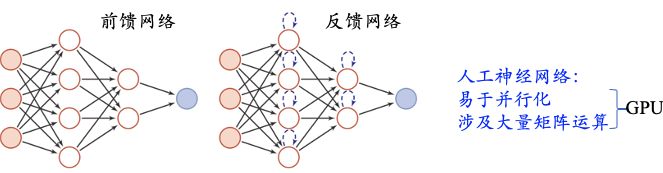
\includegraphics[width=1\textwidth]{figs/ANN2.png}
\caption{}
\label{ANN2}
\end{figure}

\subsection{ 前馈神经网络的基本结构}
% ANN 的层次结构——主要介绍神经网络的基本组成，如神经元模型、层次结构、激活函数等。这一部分强调的是网络的静态结构，即如何构造一个神经网络。
人工神经网络（ANN）通常由多个神经元（Neuron）层叠组成，每一层执行不同的计算任务。一个典型的前馈神经网络由三部分构成：
\begin{enumerate}
\item {\bf  输入层（Input Layer）} 负责接收数据，将特征输入到网络中。
\item {\bf  隐藏层（Hidden Layer）}用于提取数据的深层特征，并通过非线性变换增强网络的表达能力。
\item  {\bf  输出层（Output Layer）}根据隐藏层学习到的特征，进行最终的分类或回归预测。
\end{enumerate}

随着隐藏层的增加，神经网络的学习能力和表达能力大幅提升，使其能够处理更复杂的模式识别和预测任务。

%--
\section{深度学习（2006 及之后）：突破梯度消失，实现多层神经网络的高效训练}

针对前馈神经网络，输入层和输出层设计比较直观。针对神经网络，我们拆开想想What和How的问题：

1）神经：即神经元，什么是神经元（What）？
2）网络：即连接权重和偏置，它们是怎么连接的（How）？
对于计算机而言，它能计算的就是一些数值。而数值的意义是人赋予的。法国著名数学家、哲学家笛卡尔曾在它的著作《谈谈方法》提到：“我想，所以我是”。文雅一点的翻译就是“我思故我在”。套用在神经元的认知上，也是恰当的。这世上本没有什么人工神经元，你（人）认为它是，它就是了。也就是说，数值的逻辑意义，是人给的。

比如说，假如我们尝试判断一张手写数字图片上面是否写着数字“2”。很自然地，我们可以把图片的每一个像素的灰度值，作为网络的输入。在输入层，每个像素都是一个数值（如果是彩色图，则是3通道的数组），而把包容这个数值的容器视作一个神经元。

 输入层神经元个数的设计：如果图片的维度是16×16，那么我们输入层神经元就可以设计为256个（也就是说，输入层是一个包括256个灰度值的向量），每个神经元接受的输入值，就是归一化处理之后的灰度值。0代表白色像素，黑色像素像素代表1，灰度像素的值介于0到1之间。也就是说，输入向量的维度（像素个数）要和输入层神经元个数相同。
 
 而对输出层而言，它的神经元个数和输入神经元的个数，是没有对应关系的，而是和待分事物类别有一定的相关性。

比如说，对于图\ref{前馈神经网络的输出}所示的案例，我们的任务是识别手写数字，而数字有0~9共10类。所以，如果在输出层采用Softmax回归函数，它的输出神经元数量仅为10个，分别对应是数字“0~9”的分类概率。

最终的分类结果，择其大者而判之。比如说，如果判定为“2”的概率（比如说80\%），远远大于其他数字，那么整个神经网络的最终判定，就是手写图片中的数字是“2”，而非其它数字。

\begin{figure}[htbp]
\centering
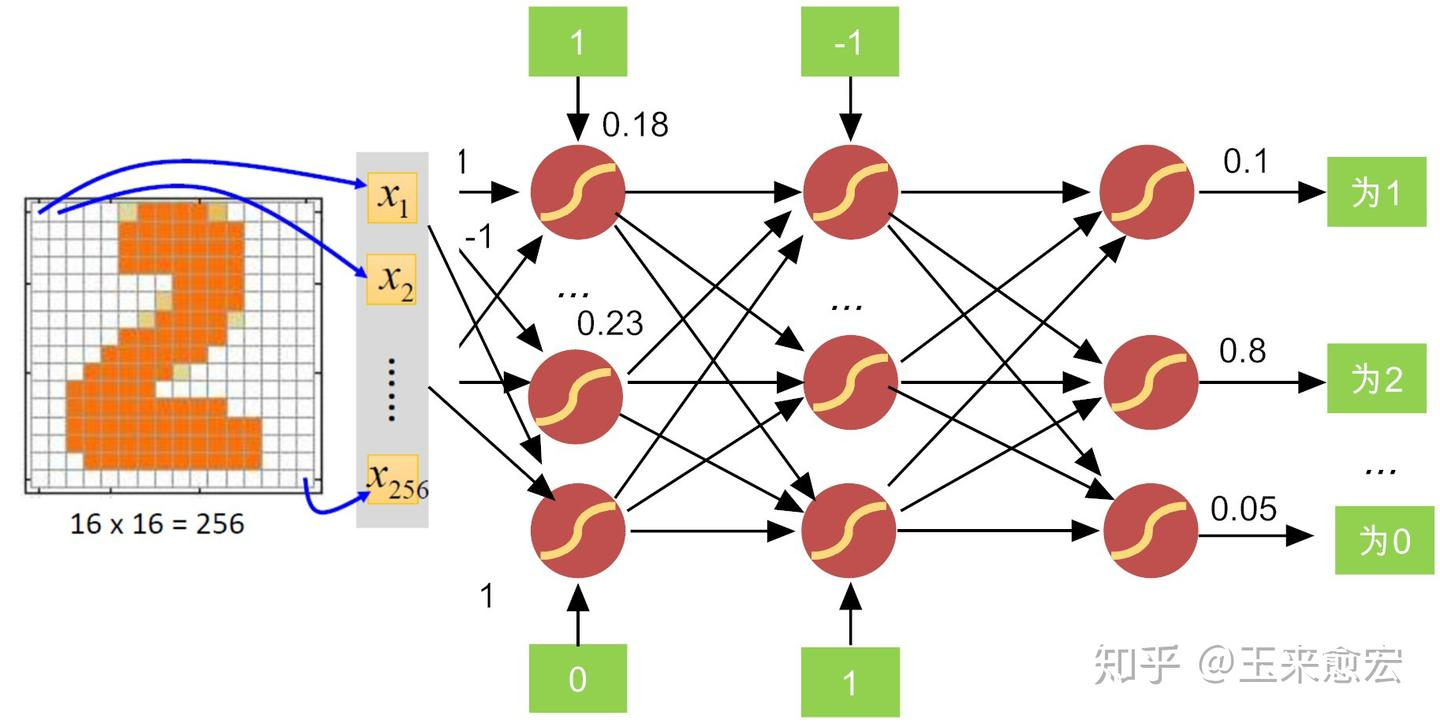
\includegraphics[width=0.69\textwidth]{figs/前馈神经网络的输出.jpg}
\caption{前馈神经网络的输出}
\label{前馈神经网络的输出}
\end{figure}

隐含层神经元个数的设计：相比于神经网络输入与输出层设计的明了直观，前馈神经网络的隐含层设计，可就没有那么简单了。说好听点，它是一门艺术，依赖于“工匠”的打磨。说不好听点，它就是一个体力活，需要不断地折腾“试错”。

我们可以把隐含层暂定为一个黑箱，它负责输入和输出之间的非线性映射变化，具体功能有点“说不清、道不明”（这是神经网络的理论短板所在）。隐含层的层数不固定，每层的神经元个数也不固定，它们都属于“超参数”，是人们根据实际情况不断调整选取的。

神经元之间是如何连接的。事实上，它同样是人赋予意义的数值参数。我们把神经元与神经元之间的影响程度叫作为权值（weight）。权重的大小就是连接的强弱。它“告诉”下一层相邻神经元更应该关注那些像素图案。

神经网络结构的设计目的在于，让神经网络以“更佳”的性能来学习。而这里的所谓“学习”，就是找到合适的权重和偏置，让损失函数的值达到最小。
%---
  
\subsubsection{ 神经元模型}
神经元（Neuron）是神经网络的基本计算单元，其核心计算包括：
%（后续可添加示意图，直观展示神经网络的计算流程）
\begin{enumerate}
\item {\bf   计算输入加权和}
每个神经元接收多个输入信号，进行加权求和：
$$
z= \sum w_i x_i +b
$$
其中，~$x_i$ 是输入， $w_i$是对应的权重（weight），$b$ 是偏置项(bias)。
这里，权重$w_i$代表神经元与神经元之间的影响程度。权重的大小就是连接的强弱。它“告诉”下一层相邻神经元更应该关注那些像素图案。

\item {\bf  通过激活函数（Activation Function）进行非线性变换}

对加权和~$z$ 施加{\bf 激活函数}的变换：
$$
y=f(z)
$$
其中 $ f(x) $ 是{\bf 激活函数}，决定神经元的输出是否被激活。
\end{enumerate}

\subsubsection{ 激活函数（Activation Function）}
激活函数的核心作用在于引入非线性，使神经网络能够学习复杂模式。如果神经网络没有激活函数，每一层的计算仅仅是线性变换的叠加，最终整个网络仍然是线性映射。这意味着无论增加多少隐藏层，网络的表达能力仍然受限。因此，非线性激活函数是神经网络突破线性限制、学习复杂函数的关键。

在所有激活函数中，阶跃函数（Step Function）和 ReLU（Rectified Linear Unit）函数的截断能力最强，它们的作用类似“开关”，决定神经元是否被激活。而其他激活函数可以被视为它们的“软化”版本，即将非连续的折线变为平滑曲线，以改善网络的学习性能。

图~\ref{activation}展示了几种常见的激活函数：
\begin{figure}[htbp]
\centering
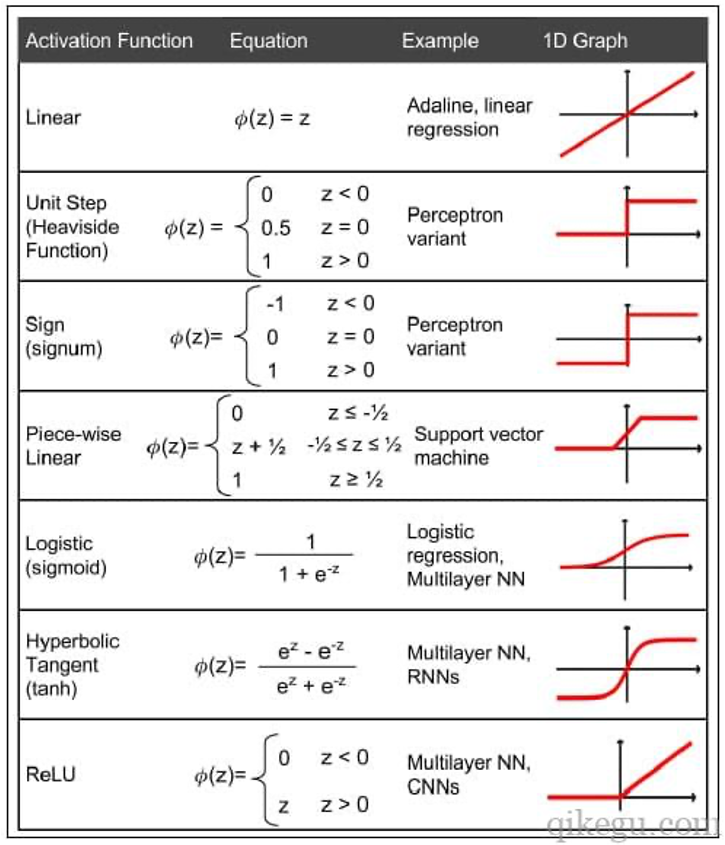
\includegraphics[width=0.8\textwidth]{figs/activation.png}
\caption{激活函数}
\label{activation}
\end{figure}

\begin{itemize}
\item {\bf 阶跃函数 (Step Function)} 
\begin{equation*}
y =\left\{ \begin{array}{ll} 
1 & \mbox{ if } x\ge 0\\
0 & \mbox{ if } x < 0\\ 
\end{array}\right.
\end{equation*} 
阶跃函数是最简单的激活函数，在早期的（单层）感知机中使用，决定神经元是否被激活。但它仅能处理线性可分问题，无法进行复杂学习。此外，由于阶跃函数非连续不可导，无法用于梯度下降优化，因此在现代神经网络中较少使用。

\item {\bf Sigmoid 函数}
$$
 f(x)= \frac{1}{1+e^{-x}}
 $$ 
 Sigmoid 函数的输出值在 (0,1) 之间，能够将输入映射到概率空间，适用于二分类任务。但它的梯度在极端值时趋于 0，容易导致梯度消失问题，训练深度网络时效果较差。
 
\item {\bf Tanh (双曲正切)函数：} 
$$f(x) = \frac{e^{x}-e^{-x}}{e^{x}+e^{-x}}$$ 
Tanh 正切函数输出范围为 (-1,1)，相比 Sigmoid 更适合归一化数据。它的梯度在 0 附近较大，收敛速度比 Sigmoid 快，但仍然容易出现梯度消失问题。  

\item {\bf ReLU（修正线性单元，Rectified Linear Unit）：}
$$
f(x)= {\rm max}(0,x)
$$
ReLU函数是目前深度神经网络中最常用的激活函数，它计算简单，不会饱和，能够有效缓解梯度消失问题。
然而，它在负半轴上的梯度恒为 0，可能导致“神经元死亡”（Dead Neuron）现象，即某些神经元的输出永远为 0，不再更新参数。

\item {\bf Leaky ReLU (带泄漏的 ReLU)}
\begin{equation*}
y =\left\{ \begin{array}{ll} 
x & \mbox{ if } x\ge 0\\
\alpha x & \mbox{ if } x < 0\\ 
\end{array}\right.
\end{equation*} 
Leaky ReLU 在负半轴引入了一个小的非零斜率~$\alpha$（通常取 0.01），使得负值区域时神经元在仍然能接收梯度更新，减少神经元死亡问题。

\item {\bf Softmax 函数}
$$f(x_i) = \frac{e^{x_i}}{ \sum e^{x_j}}$$

 Softmax 函数适用于多分类任务，能够将输出归一化的概率分布，使得所有类别的概率总和为 1，便于模型进行分类决策。   
\end{itemize}

激活函数在神经网络中起着至关重要的作用，它决定了网络的非线性映射能力，影响梯度传播的稳定性以及计算效率。
激活函数的设计需要平衡以下几个关键因素：
\begin{enumerate}
\item {\bf  可导性（Differentiability）：} 由于梯度下降法（Gradient Descent）用于优化神经网络，需要对激活函数求导，因此激活函数应在定义域内保持可微。早期感知机（Perceptron）使用的 阶跃函数（Step Function） 仅能输出 0 或 1，不连续不可导，无法用于梯度优化。
\item {\bf  梯度稳定性（Gradient Stability）： }选择适当的激活函数能够避免梯度消失（Vanishing Gradient）或梯度爆炸（Exploding Gradient）问题，从而确保深度网络能够有效训练。例如，Sigmoid 和 Tanh 函数 在极端值区域会导致梯度接近零，影响网络学习，而 ReLU 函数 及其变体在深度学习中表现更优。
\item {\bf  计算效率（Computational Efficiency）：} 计算简单的激活函数能够加速网络的训练。ReLU 及其变体（Leaky ReLU、PReLU） 计算量较小，相比 Sigmoid 和 Tanh 具有更好的数值稳定性，成为深度神经网络的主流选择。
\end{enumerate}

选择合适的激活函数对于训练稳定性、收敛速度和最终模型的性能有着至关重要的影响。
不同任务需要选择合适的激活函数，以确保网络能够高效学习并避免梯度消失或梯度爆炸等问题。 在实际应用中，对于回归任务，常用 ReLU 或 Tanh 作为隐藏层激活函数，因为它们能够输出连续值；对于二分类任务，通常使用 Sigmoid 作为输出层激活函数，因为其输出值在~$(0,1)$ 之间，可以解释为概率；对于多分类任务，Softmax 是最优选择，能够将输出归一化为概率分布；
深度神经网络的隐藏层通常使用 ReLU 或 Leaky ReLU，以避免梯度消失，提高训练效率。

\subsection{前馈神经网络的学习过程}
神经网络的学习过程本质上是一个{\bf 参数优化问题}，目标是不断调整网络的权重参数，使输出尽可能接近真实值。

本节，我们以监督学习（Supervised Learning）为例 ，详细描述神经网络的学习过程。在无监督学习（Unsupervised Learning）和半监督学习（Semi-Supervised Learning）中，神经网络的训练方式有所不同，我们将在后续章节详细讨论它们的学习范式。

在监督学习任务中，神经网络的学习过程通常由{\bf 前向传播(Forward Propagation、误差计算(Loss Computation)、反向传播(Backpropagation)和权重更新(Weight Update)}四个阶段构成。

\begin{enumerate}
\item {\bf  前向传播（Forward Propagation）：} 数据在网络中向前逐层传递，经过加权求和和激活函数变换等神经元计算，生成输出预测值。
\item {\bf  计算损失（Loss Computation）： }评估预测结果与真实标签之间的误差，使用损失函数进行衡量。
\item {\bf  误差反向传播（Backpropagation）：} 误差从输出层向隐藏层反向传播，计算各层权重对损失的梯度。
\item {\bf  权重更新（Weight Update）：} 通过优化算法（如梯度下降）调整网络权重，使模型在下一次迭代中表现得更好。
\end{enumerate}

接下来，我们详细探讨这四个阶段。

\subsubsection*{前向传播（Forward Propagation）}
神经网络的前向传播是神经网络的计算流程，输入数据从输入层开始，逐层流向隐藏层，最终到达输出层。

不失一般性，我们假设神经网络仅有一个隐藏层。假设神经网络的输入层有~$m$ 个特征 ，表示为 $X = (x_1, x_2, \dots, x_m)$，隐藏层包含 $p$ 个神经元，表示为 $H = (h_1, h_2, \dots, h_p)$，输出层包含 $n$ 个神经元，表示为 $Y = (y_1, y_2, \dots, y_n)$。神经网络的权重矩阵由两部分组成，分别是输入层到隐藏层的权重矩阵 $W = (W_{ij})_{m\times p}$  和 隐藏层到输出层的权重矩阵 $V = (V_{jk})_{p\times n}$，其中~$ W_{ij} $ 为连接输入 $ x_i $ 和隐藏层神经元 $ h_j $，$ V_{jk} $ 为连接隐藏层 $ h_j $ 和输出神经元 $ y_k $， $b_j$ 和 $c_k$ 分别为隐藏层神经元~$h_j$ 和输出层神经元~$y_k$ 的偏置项。

在前向传播过程中，输入层的数据~$X$ 首先与权重 $W$ 进行加权求和，并添加偏置项 $b_j$，然后通过激活函数 $f(x)$ 进行非线性变换，得到隐藏层的输出：
$$ h_j = f\left( \sum_{i=1}^m W_{ij} x_i +b_j \right), \quad j=1,2,\dots, p$$
其中 $ f(x) $ 是隐藏层的{\bf 激活函数}，如 ReLU 或 Sigmoid。。

接下来，隐藏层的输出继续传递到输出层。每个输出神经元同样对隐藏层的输出进行加权求和，并添加偏置项 $c_k$，然后通过输出层的激活函数 $g(x)$ 计算最终的预测值：
$$ \hat y_k = g\left( \sum_{j=1}^p V_{jk} h_j +c_k \right), \quad k=1,2,\dots, n$$
其中 $ g(x) $ 是输出层的激活函数，常见的选择包括 Sigmoid（用于二分类任务）和 Softmax（用于多分类任务）。

网络的预测输出~$\hat Y= ( \hat{y_1},\hat{y_2},\dots,\hat{y_n} )$ 作为模型的输出，与真实标签 $Y = (y_1, y_2, \dots, y_k)$ 进行比较，以计算损失，从而指导下一步的优化过程。

\subsubsection*{计算损失（Loss Computation）}

在前向传播过程中，神经网络根据输入数据计算出预测值 $\hat{Y} = (\hat{y_1}, \hat{y_2}, \dots, \hat{y_k})$，但由于模型的初始权重是随机设定的，预测值 $\hat{Y}$ 可能与真实值 $Y = (y_1, y_2, \dots, y_k)$ 存在较大的误差。为了衡量这种误差，我们需要定义 损失函数（Loss Function），以量化预测结果与真实标签之间的偏差，指导后续的权重更新。

损失函数 $L$ 的目标是最小化预测值 $\hat{Y}$ 和真实值 $Y$ 之间的误差。不同的任务类型适用于不同的损失函数。在监督学习中，最常见的任务是 回归（Regression） 和 分类（Classification），它们通常采用不同的损失函数来度量误差。

对于回归任务，目标是预测一个连续的数值，因此损失函数通常采用 均方误差（Mean Squared Error, MSE）：
$$ L = \frac{1}{2} \sum_{k=1}^K \left( y_k-\hat y_k \right)^2, $$
其中~$y_k$是真实值，~$\hat y_k$是预测值。 均方误差衡量了预测值 $\hat{y_k}$ 与真实值 $y_k$ 之间的平方差，并对所有输出求和后取平均。平方的作用是让误差对大偏差更加敏感，同时保持导数的连续性，使得优化更稳定。

除了均方误差，有时也会使用 均方根误差（Root Mean Squared Error, RMSE）:
$$
L= \sqrt{\frac{1}{K} \sum_{k=1}^K \left( y_k-\hat y_k \right)^2}
$$
或者 平均绝对误差（Mean Absolute Error, MAE）：
$$
L=\frac{1}{K}  \sum_{k=1}^K \left( y_k-\hat y_k \right|
$$
其中，MAE 计算的是预测值与真实值之间的绝对误差，鲁棒性较强，但对大误差的敏感度低于 MSE。

而在分类任务中，输出层通常是一个概率分布，我们希望模型预测出的概率尽可能接近真实类别的概率。为此，常采用交叉熵损失（Cross-Entropy Loss），它能够衡量两个概率分布之间的差异，并通过放大低概率类别的损失来加速模型的收敛。此外，交叉熵的梯度更适合优化，使得模型在训练过程中能够更稳定地更新权重。

对于二分类问题，交叉熵损失定义如下：
$$
L= -\sum_{k=1}^K y_k\, {\rm log } \hat y_k + (1-y_k) \, {\rm log } (1-\hat y_k).
$$
其中，$\hat{y_k}$ 是模型预测的类别概率，$y_k$ 是真实类别标签（0 或 1）。交叉熵损失能够度量模型在概率预测上的不确定性，当预测值 $\hat{y_k}$ 越接近真实值 $y_k$，损失越小。

对于多分类任务，交叉熵损失的形式推广为：
$$
L= -\sum_{k=1}^K y_k\, {\rm log } \hat y_k.
$$
在该公式中，$y_k$ 是独热编码（one-hot encoding）形式的真实标签，$\hat{y_k}$ 是模型预测的 Softmax 输出概率。该损失能够衡量整个分类任务的误差，使得模型趋向于正确分类样本。

通过计算损失函数 $L$，我们得到了模型的当前误差。下一步，我们将利用反向传播（Backpropagation） 算法，计算损失函数关于网络权重的梯度，以指导权重的更新，优化模型的预测能力。

\subsubsection*{ 误差反向传播（Backpropagation）} 
在计算损失后，神经网络需要调整参数，以使预测结果更接近真实值。
这一过程依赖于{\bf 误差反向传播（Backpropagation, BP）}，它是一种基于{\bf 梯度下降（Gradient Descent）}的优化方法，用于计算损失函数对每个权重的梯度，并逐层更新网络参数，以最小化预测误差。

梯度下降的核心思想是{\bf 沿着损失函数下降最快的方向调整参数}，从而优化模型性能。具体来说，它首先计算损失对输出层的影响，然后 逐层反向传播误差信息，计算各层参数对最终误差的贡献，并据此调整权重，使所有参数都能基于它们对整体误差的影响进行合理优化。

误差反向传播是一种高效的梯度计算方法，它通过{\bf 链式法则（Chain Rule）}计算误差在网络中的传播方式，使得误差能够从输出层逐层反向传播至输入层，并高效计算每个权重的调整量。

具体而言，
\begin{enumerate}
\item {\bf  计算输出层的误差}

由于损失函数 $L$ 依赖于网络的输出 $\hat{y_k}$，首先计算输出层的误差：
$$
\delta_k = \left( y_k-\hat y_k \right)g^\prime(\hat y_k)
$$
其中，$y_k$ 是真实标签，$\hat{y_k}$ 是网络的预测值，$g^\prime(\hat{y_k})$ 是输出层激活函数的导数，用于衡量输出层的梯度变化。

直观来看，如果预测值 $\hat{y_k}$ 远离真实值 $y_k$，那么误差项 $\delta_k$ 会较大，导致较大的梯度，从而驱动参数向减少误差的方向调整；反之，如果预测已经接近真实值，则误差项较小，参数的更新幅度也会相应减小。

\item {\bf 计算隐藏层的误差项}
由于隐藏层的输出直接影响输出层，因此需要计算隐藏层对最终损失的贡献，并将误差从输出层反向传递到隐藏层：
$$
\delta_j = \left(\sum_j V_{jk} \delta_k  \right)f^\prime(h_j)
$$
其中，$V_{jk}$ 是隐藏层到输出层的权重矩阵，$\delta_k$ 是从输出层传播回来的误差，$f^\prime(h_j)$ 是隐藏层激活函数的导数，衡量隐藏层的输出变化对最终误差的影响。

这一计算的直观含义是，如果某个隐藏层神经元对多个输出神经元都有较大的权重连接（即 $V_{jk}$ 较大），那么它对误差的贡献就更显著，因此它的梯度应该相应增大。
\end{enumerate}

\subsubsection*{权重更新（Weight Update）}

基于上一步计算出的梯度，我们利用{\bf 梯度下降算法（Gradient Descent）}或其变体方法（如 Adam, RMSprop）来更新权重，使得网络在下一次迭代时能够产生更准确的预测。

{ 在误差反向传播到隐藏层之后，计算每个权重参数对损失函数的影响，并利用梯度下降来更新权重：
$$
 \frac{\partial L}{\partial V_{jk}}=\delta_k h_j 
$$
$$
 \frac{\partial L}{\partial W_{ij}}=\delta_j x_i 
$$
其中，$h_j$ 是隐藏层的激活值，$x_i$ 是输入层的输入数据。

这意味着，隐藏层到输出层的权重更新量 取决于隐藏层的输出 $h_j$ 以及输出层的误差项 $\delta_k$，而输入层到隐藏层的权重更新量 取决于输入数据 $x_i$ 以及隐藏层的误差项 $\delta_j$。

通过这些步骤，神经网络可以计算出如何调整每个权重，以最小化预测误差。}

在传统梯度下降方法中，使用的是基本的权重更新规则：
$$
V_{jk}^{(t+1)} =V_{jk}^{(t)} +\eta \delta_k h_j
$$
$$
W_{ij}^{(t+1)} =W_{ij}^{(t)} +\eta \delta_j x_i
$$
其中~$\eta$是学习率(learning rate)，决定了更新步长，~$V_{jk}$ 是隐藏层到输出层的权重，$ W_{ij} $ 是输入层到隐藏层的权重，$\delta_k$ 和 $\delta_j$ 分别是输出层和隐藏层的误差项。

学习率 $\eta$ 是神经网络训练中的关键超参数，决定了参数的更新步长。如果学习率过大，更新步长过长，可能导致梯度 剧烈震荡 或 无法收敛；反之，如果学习率过小，更新步长过短，可能导致 收敛速度慢 或 陷入局部最优。通常，我们会使用 学习率衰减（Learning Rate Decay） 技术，在训练过程中 逐步降低学习率，以保证更稳定的收敛。

\subsubsection*{梯度下降方法及其变体}
在神经网络的训练过程中，梯度下降（Gradient Descent）是一种核心优化方法，其目标是最小化损失函数 \( L \) 以优化模型参数 \( \theta \)。梯度下降的更新规则如下：
\begin{equation}
\theta^{(t+1)} = \theta^{(t)} - \eta \frac{\partial L}{\partial \theta}
\end{equation}
其中，\(\eta\) 为学习率（learning rate），决定了每次参数更新的步长。

不同的梯度下降策略影响计算效率、收敛速度和最终的优化性能。根据计算梯度所使用的数据量不同，梯度下降方法主要分为三种：批量梯度下降（BGD）、随机梯度下降（SGD）和小批量梯度下降（Mini-batch SGD）。

\paragraph*{批量梯度下降（Batch Gradient Descent, BGD)}
批量梯度下降在每次迭代时计算整个训练集上的损失函数平均梯度，并基于该平均梯度更新参数：
\begin{equation}
\theta^{(t+1)} = \theta^{(t)} - \eta \frac{1}{N} \sum_{i=1}^{N} \frac{\partial L_i}{\partial \theta}
\end{equation}
其中，\(N\) 是训练样本的总数，\(\frac{\partial L_i}{\partial \theta}\) 是第 \(i\) 个样本的梯度。

这种方法保证了梯度更新的稳定性，优化路径不会受随机噪声影响。然而，它需要在每次更新时计算整个训练集的梯度，在数据量较大时，计算开销较高，并且当数据集包含大量冗余信息时，计算效率较低。因此，尽管批量梯度下降具有全局稳定的优化方向，但它不适用于大规模数据集。

\paragraph*{随机梯度下降（Stochastic Gradient Descent, SGD)}
随机梯度下降在每次更新时仅使用一个训练样本计算梯度：
\begin{equation}
\theta^{(t+1)} = \theta^{(t)} - \eta \frac{\partial L_i}{\partial \theta}
\end{equation}
其中，\( L_i \) 是训练集中某个随机抽取的样本的损失。

随机梯度下降使得参数能够更快地进行更新，提高了计算效率，并避免了因冗余数据而导致的计算浪费。然而，由于每次更新仅依赖单个样本的梯度，随机梯度下降 会导致优化路径的剧烈波动，可能使参数在损失函数的局部最优点附近振荡，而难以稳定收敛。因此，在实际应用中，随机梯度下降需要结合学习率衰减或其他优化方法来提高收敛效果。

\paragraph*{小批量梯度下降（Mini-batch SGD）}
小批量梯度下降在每次迭代时在一个小批量（Mini-batch）样本来计算梯度：
\begin{equation}
\theta^{(t+1)} = \theta^{(t)} - \eta \frac{1}{m} \sum_{i=1}^{m} \frac{\partial L_i}{\partial \theta}
\end{equation}
其中，\(m\) 是小批量的大小，通常设置为 32、64 或 128。

小批量梯度下降结合了批量梯度下降的稳定性和随机梯度下降的计算效率，既能提高计算速度，又能减少梯度更新的波动，使训练更加稳定。由于其在大规模数据集上的良好适应性，目前小批量梯度下降是深度学习中最常用的优化方法。

%\subsection{自适应优化方法}
除了基本的梯度下降方法，研究者们还提出了一些自适应优化算法，它们能够动态调整学习率，以提高收敛速度和训练稳定性。这些方法在深度学习中得到了广泛应用。

\paragraph*{动量法（Momentum）}
动量法（Momentum）在梯度下降的基础上引入一个历史梯度的累积项，使得参数更新方向更加稳定，并减少震荡。其更新公式如下：
\begin{equation}
v^{(t+1)} = \beta v^{(t)} + (1-\beta) \frac{\partial L}{\partial \theta}
\end{equation}
\begin{equation}
\theta^{(t+1)} = \theta^{(t)} - \eta v^{(t+1)}
\end{equation}
其中，\( v^{(t)} \) 代表梯度的指数加权平均，\( \beta \) 是动量因子，通常取 \( 0.9 \)。当梯度更新方向相对一致时，动量法可以加速收敛；而当梯度方向变化较大时，它能平滑优化路径，减少震荡。

\paragraph*{RMSprop（Root Mean Square Propagation）}
RMSprop 通过指数加权平均的方式动态调整学习率，以适应不同参数的梯度变化。其核心思想是对梯度的二阶矩进行指数平滑：
\begin{equation}
s^{(t+1)} = \beta s^{(t)} + (1-\beta) \left(\frac{\partial L}{\partial \theta} \right)^2
\end{equation}
\begin{equation}
\theta^{(t+1)} = \theta^{(t)} - \frac{\eta}{\sqrt{s^{(t+1)} + \epsilon}} \frac{\partial L}{\partial \theta}
\end{equation}
其中，\( \epsilon \) 是一个小数值（如 \(10^{-8}\)），用于避免分母为零的情况。RMSprop 适用于非平稳目标函数，特别是在时间序列任务中表现优越，如循环神经网络（RNN）的训练。

\paragraph*{Adam（Adaptive Moment Estimation）}
Adam 结合了 Momentum 和 RMSprop 方法，能够自适应调整每个参数的学习率，是目前最常用的优化算法之一。其更新规则如下：
\begin{equation}
m^{(t+1)} = \beta_1 m^{(t)} + (1-\beta_1) \frac{\partial L}{\partial \theta}
\end{equation}
\begin{equation}
s^{(t+1)} = \beta_2 s^{(t)} + (1-\beta_2) \left(\frac{\partial L}{\partial \theta} \right)^2
\end{equation}
\begin{equation}
\hat{m}^{(t+1)} = \frac{m^{(t+1)}}{1 - \beta_1^t}, \quad \hat{s}^{(t+1)} = \frac{s^{(t+1)}}{1 - \beta_2^t}
\end{equation}
\begin{equation}
\theta^{(t+1)} = \theta^{(t)} - \frac{\eta}{\sqrt{\hat{s}^{(t+1)} + \epsilon}} \hat{m}^{(t+1)}
\end{equation}
其中，\( \beta_1 \) 和 \( \beta_2 \) 分别控制梯度一阶矩和二阶矩的衰减速率，默认值通常为 \(0.9\) 和 \(0.999\)。

关于这些自适应优化方法的更详细介绍，请参考~\cite{kingma2014adam,bengio2012practical}：

%在无监督学习和半监督学习中，神经网络的训练方式不同，我们将在后续章节会详细讨论它们的学习范式。

\subsection{ 神经网络的数学灵魂：通用逼近定理（Universal Approximation Theorem）}

神经网络的核心目标是{\bf 学习并逼近复杂函数}，无论是图像识别、语音处理，还是预测模型，最终都可以抽象为一个数学问题：{\bf 找到一个合适的函数，使其能够精准地映射输入到输出}。然而，神经网络是否具备逼近任何函数的能力？通用逼近定理（Universal Approximation Theorem, UAT） 正是对这个问题的回答。

从数学角度来看，单纯的线性变换是无法表达复杂模式的。若神经网络不包含激活函数，那么无论增加多少层，其整体仍然是线性变换的堆叠。而线性变换的组合仍然是线性变换，因此，这种神经网络最终只能学习一个线性映射，无法解决非线性问题。这意味着，单纯的加深网络并不会提升模型的表达能力。为了使神经网络能够逼近复杂的模式，必须引入非线性激活函数。

通用逼近定理（Universal Approximation Theorem, UAT）由 Cybenko（1989） 和 Hornik 等人（1989）~\cite{hornik1990universal, cybenko1989approximation,}” 提出，描述如下：

{\em “任何具有至少一个非线性激活函数的单隐藏层前馈神经网络，只要隐藏层神经元的数量足够，可以以任意精度近似任何定义在实数域上的有界闭集函数。”}

换句话说，{\bf 单隐藏层神经网络非常强大，理论上可以逼近任何连续函数。}只要隐藏层的神经元足够多，并调整合适的权重，总能找到一个网络，使其输出无限接近于目标函数。
这一理论为神经网络的表达能力提供了数学保证，也解释了为什么深度学习能够在各种复杂任务中大放异彩。

\begin{figure}[htbp]
\centering
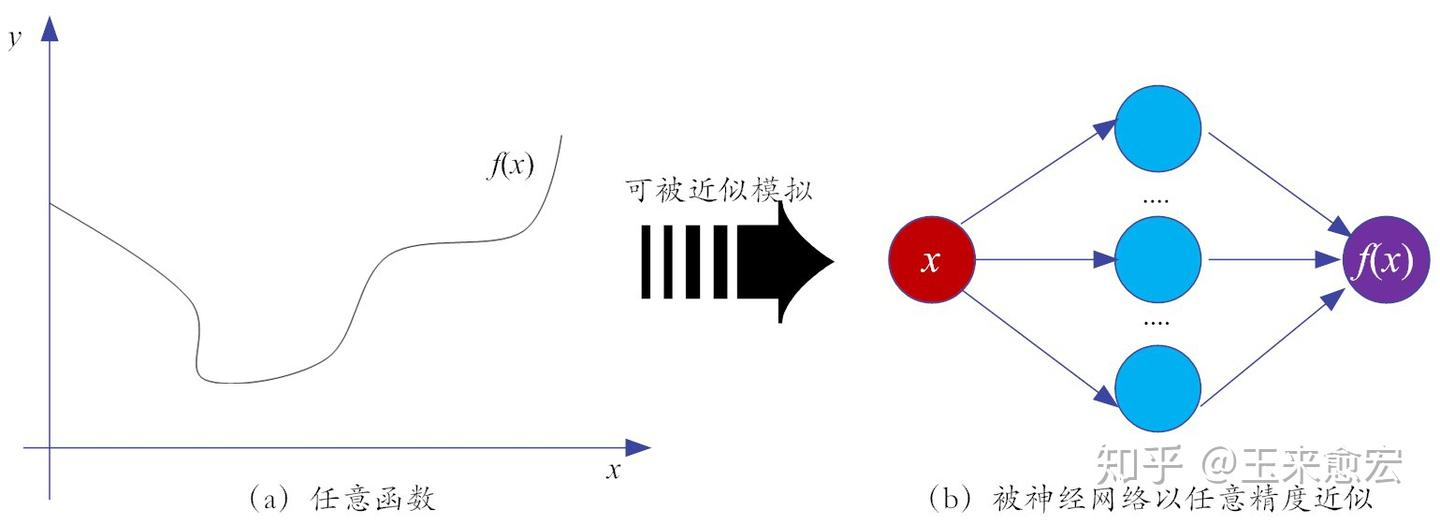
\includegraphics[width=1\textwidth]{figs/通用逼近定理.jpg}
\caption{通用逼近定理}
\label{通用逼近定理}
\end{figure}

\subsubsection*{通用逼近定理的直觉理解}
通用逼近定理听起来近乎神奇，因此也常被称为“万能逼近定理”。
它的数学证明基于神经网络的分段逼近（piecewise approximation）思想。直观上，任何复杂的非线性函数都可以拆解为多个局部线性片段，而神经网络通过激活函数的非线性变换，能够灵活地拼接这些片段，从而形成复杂的全局映射。

激活函数是神经网络的“非线性源泉”。
在没有激活函数的情况下，神经网络的每一层只是对输入数据进行线性变换，无论如何堆叠隐藏层，最终只能拟合线性关系，无法有效表达非线性函数。
因此，激活函数的引入至关重要。

正如激活函数的名字“activation”所言，激活函数的作用可以理解为提供局部的“打开-关闭”机制，使得神经网络可以在不同的输入区域内学习不同的映射关系。
以 ReLU（修正线性单元）为例，输入~$x<0$时，输出~$y= 0$，相当于“截断(关闭)”功能；而输入~$x>0$ 时，输出~$y=x$， 相当于“导通(打开)”功能。而Sigmoid/Tanh 等激活函数具有“挤压”性质，能够将输入映射到特定区间，从而增强神经网络的非线性表达能力。

通过这些激活函数，神经网络可以在不同输入区域内应用不同的线性变换，最终在全局上形成非线性映射，逼近任意目标函数。\footnote{如果将神经网络的逼近能力与数学分析中的方法进行类比，它的核心思想与傅里叶级数逼近定理极为相似。
傅里叶级数通过一系列正弦波的叠加来逼近任何复杂的周期函数，而神经网络 通过多个非线性激活单元的组合，来逼近任意复杂的连续函数。
换句话说，神经网络可以看作是“数据驱动的傅里叶级数”，这正是它能够广泛应用于图像识别、自然语言处理等复杂任务的数学基础。}

%\subsubsection{示例：神经网络逼近 $f(x) = \sin(x)$}尝试用神经网络拟合一个分段函数：由3段直线组成
%本节，我们提供一个神经网络可以逼近任何函数的简单示例。示例来自于Michael Nielsen的博客文章~\cite{nielsen2015neural} 。%可视化证明
%
%假设我们希望训练一个简单的前馈神经网络来逼近非线性函数 $ f(x) = \sin(x) $ 。直观上，$\sin(x)$ 具有周期性和非线性特性，而单纯的线性变换无法准确拟合它。
%
%1. 选择输入和输出：输入~$x$（单个实数），目标输出~$y = {\rm sin}(x)$。 
%
%2. 选择神经网络结构：
%我们使用一个单隐藏层的神经网络，其结构如下：
%\begin{itemize}
%\item {\bf  输入层：} 单个神经元 (输入 $ x $)
%\item {\bf  隐藏层：} $10 $ 个神经元，每个神经元使用Sigmoid作为激活函数
%\item {\bf  输出层：} 单个神经元，输出预测值 $\hat{y}$作为对~${\rm sin}(x)$ 的近似
%\end{itemize}
%
%3. 神经网络计算过程：
%隐藏层计算（假设使用 Sigmoid 激活函数）：
%$$
%h_j = \sigma (w_i x_i +b_j), \quad j=1,2,\dots, 10,
%$$
%其中~$w_j$ 和~$b_j$​ 是隐藏层的权重和偏置，~$\sigma(x)= \frac{1}{1+e^{-x}}$ 是 Sigmoid 激活函数。
%
%输出层计算（线性组合隐藏层神经元的输出）：
%$$
%\hat y = \sum_{j=1}^{10} v_j h_j+c  
%$$
%其中~$v_j$ 是输出层的权重，~$c$ 是输出层的偏置。
%
%4. 训练网络：
%
%输入~$x$ 在区间~$[-\pi, \pi]$  采样 10 个数据点。
%(1) 定义损失函数
%我们采用 均方误差 (MSE) 作为损失函数计算预测值~$\hat y $ ​ 与真实值~$y$ 之间的误差:
%$$
%L= \frac{1}{10} \sum_{i=1}^{10} \left(  {\rm sin}(x_i) -\hat y_i\right)^2
%$$
%
%均方误差度量了预测值与真实值之间的平方差，并取平均值。当预测值~$\hat y_i$  远离真实值~${\rm  sin}(x)$ 时，损失较大，促使网络进行更大幅度的权重调整；而当预测值逐渐接近真实值时，损失降低，使网络在学习过程中趋于收敛。
%
%采用 梯度下降或 Adam 优化算法 训练网络，调整~$w_j, b_j, v_j, c$ 使得~$\hat y$ 逼近~${\rm sin}(x)$。 
%
%训练后，该神经网络可以在~$[-\pi, pi]$ 范围内很好地拟合~${\rm sin}(x)$曲线，尽管它使用的是 简单的线性组合 + 非线性激活，但由于通用逼近定理（Universal Approximation Theorem），单隐藏层已经足够逼近这个非线性函数。
%
%如果增加隐藏层的神经元数量或使用 更深的网络，则可以进一步提升拟合精度，使得神经网络在更大范围内更好地逼近~${\rm sin}(x)$。
%
%设定学习率$\eta = 0.01$。
%
%不同优化方法的训练轮数
%梯度下降（Gradient Descent, GD）：由于梯度下降在小批量数据上收敛较慢，预计 3000 - 5000 轮 可达到较好的逼近效果。训练初期可能会出现损失下降较慢的情况，需要耐心等待。
%
%Adam 优化器：Adam 由于自适应学习率的优势，通常可以在 1000 - 2000 轮 训练后得到较好的拟合。
%如果隐藏层神经元足够多（如~$m=20$），则可能 500 - 1000 轮 即可达到较低损失。
%
%早停策略（Early Stopping）：在每 100 轮迭代后计算验证损失，并监测收敛情况。
%若损失在 连续 200 轮内没有显著下降，可以提前终止训练，通常能在 1000 - 1500 轮 内收敛。
%损失曲线（Loss Curve）在训练过程中，我们可以记录损失值~$L$ 并绘制损失曲线，以观察训练的收敛趋势：
%前 500 轮: 损失下降较快，神经网络逐步学习到正弦函数的趋势。
%500 - 1500 轮: 进一步优化，细节拟合逐渐完善。
%1500 轮以后: 若损失下降幅度变小，可以考虑提前停止训练。
%最终预测效果
%训练足够轮次后，测试数据的输出 ~$\hat 𝑦$ 会接近~${\rm  sin}(x)$，并呈现较好的拟合效果。对于简单的 10 个数据点，最终拟合误差~$L$ 可以接近~$ 10^{-3}$ 甚至更小。
%  
%下图展示了不同数量的隐藏层神经元对 $\sin(x)$ 逼近的效果：
%
%少量神经元（如 $n=3$）时，网络只能学到几个折线段，近似效果较差。
%增加神经元数量（如 $n=10$），网络可以更精细地学习曲线结构，逼近效果大幅提升。
%理论上，当 $n \to \infty$ 时，神经网络可以无限逼近 $\sin(x)$，这正是通用逼近定理的直观体现。
%
%% 以下代码使用 Keras 训练一个单隐藏层的神经网络来拟合 $\sin(x)$：
%%import numpy as np
%%import matplotlib.pyplot as plt
%%from tensorflow import keras
%%from tensorflow.keras import layers
%%
%%# 生成训练数据
%%x_train = np.linspace(-2*np.pi, 2*np.pi, 1000)
%%y_train = np.sin(x_train)
%%
%%# 构建神经网络
%%model = keras.Sequential([
%%    layers.Dense(10, activation="relu", input_shape=(1,)),  # 单隐藏层，10个神经元
%%    layers.Dense(1)  # 输出层
%%])
%%
%%# 编译模型
%%model.compile(optimizer="adam", loss="mse")
%%
%%# 训练模型
%%model.fit(x_train, y_train, epochs=100, verbose=0)
%%
%%# 预测
%%y_pred = model.predict(x_train)
%%
%%# 绘制结果
%%plt.plot(x_train, y_train, label="True $\sin(x)$", linestyle="dashed")
%%plt.plot(x_train, y_pred, label="NN Approximation", color="red")
%%plt.legend()
%%plt.show()

\section{人工神经网络的主要类型}
在上一节中，我们介绍了前馈神经网络（FNN），它是最基础的人工神经网络结构，也是多层感知机（MLP）的扩展形式。FNN 通过 前向传播 计算输出，并使用 误差反向传播（Backpropagation） 进行训练，最终调整权重参数，使得网络能够逼近目标函数。

然而，前馈神经网络并不能解决所有任务。随着研究的深入，科学家们提出了多种不同结构的神经网络，以适应不同的数据特性和应用场景。根据 {\bf 拓扑结构} 和 {\bf 信息传播方式}，人工神经网络可以大致分为以下几类：

\paragraph*{ 前馈神经网络（Feedforward Neural Networks, FNN）}

前馈神经网络（Feedforward Neural Networks, FNN）
前馈神经网络是 {\bf 最基础} 的神经网络结构，它由 输入层、隐藏层和输出层 组成。数据在网络中按照单向流动的方式传播，并不会在层之间形成循环连接。FNN 适用于静态数据处理，例如图像分类和回归任务。由于其结构相对简单，训练相对稳定，因此在许多传统机器学习任务中得到了广泛应用。多层感知机（MLP）是 FNN 的典型代表，它通过增加隐藏层的数量，使得网络能够学习更加复杂的非线性映射。然而，由于缺乏循环连接，前馈神经网络难以处理时间序列数据，这种局限性促使研究者提出了 递归神经网络（RNN） 来建模时间相关的信息。

\paragraph*{ 循环神经网络（RNN）}
与前馈神经网络不同，递归神经网络允许信息在网络中循环传播，使得当前时刻的输出可以受到之前时刻输入的影响。因此，RNN 适用于处理时间序列数据，例如语音、文本和金融数据预测。它能够利用隐藏状态来存储过去的信息，并结合当前输入进行计算，从而建模序列数据中的时间依赖性。然而，传统 RNN 在长序列任务中容易遭遇梯度消失或梯度爆炸问题，导致网络难以学习较长时间跨度的信息。为了缓解这一问题，研究者提出了{\bf  长短时记忆网络（LSTM）} 和 {\bf 门控循环单元（GRU）}，它们通过设计门机制来控制信息的流动，从而有效提升了模型的长期依赖学习能力。RNN 及其变种广泛应用于机器翻译、语音识别和文本生成等任务。

\paragraph*{ 卷积神经网络（CNN）}
卷积神经网络专门用于处理 图像和其他网格状数据，它通过 {\bf 局部连接} 和 {\bf 权重共享} 方式减少计算量，并提高模型对位移、旋转和缩放变化的学习能力。CNN 由 {\bf 卷积层、池化层和全连接层} 组成，其中卷积层通过滑动窗口的方式提取局部特征，池化层进一步降低计算复杂度并提高模型的泛化能力。CNN 在计算机视觉领域取得了革命性的突破，成为目标检测、人脸识别和医学影像分析等任务中的核心模型。随着研究的深入，CNN 逐步发展出 ResNet、DenseNet 和 MobileNet 等变体，使得网络在深度增加的同时，仍然能够保持较高的训练效率和泛化能力。

\paragraph*{ 自编码器（Autoencoder, AE）} 
自编码器是一种 {\bf 无监督学习} 的神经网络，其目标是学习输入数据的低维表示，并尽可能保留关键信息。该网络由 {\bf 编码器（Encoder） 和 解码器（Decoder）} 组成，编码器负责将输入数据映射到低维表示，而解码器则尝试从低维表示中重建原始输入。自编码器可以用于{\bf  数据降维、特征提取和异常检测}，并且在生成模型和数据压缩等领域具有广泛的应用。变分自编码器（VAE）是自编码器的一种扩展形式，它在编码过程中引入了概率分布的约束，从而使得生成的数据更加多样化和稳定。

\paragraph*{生成对抗网络（Generative Adversarial Networks, GAN）  }
生成对抗网络由 {\bf 生成器（Generator） 和 判别器（Discriminator） }组成，二者通过对抗训练 进行优化，最终使得生成器能够生成逼真的合成数据，而判别器则不断提高对真实数据和生成数据的辨别能力。GAN 的核心思想在于让生成器和判别器进行博弈，使得生成器最终可以生成难以区分的高质量数据。GAN 在图像生成、风格迁移和数据增强等领域取得了突破性的成果，被广泛应用于 AI 艺术、DeepFake 和医学图像合成等任务。然而，由于 GAN 训练的不稳定性和模式崩溃（mode collapse）问题，研究者提出了 WGAN、StyleGAN 和 BigGAN 等改进模型，以提升训练的稳定性和生成数据的质量。

\paragraph*{其他神经网络架构}
除了上述主要类型的神经网络外，研究者还提出了适用于不同数据结构和任务的特殊网络架构。例如，{\bf 变分自编码器（VAE）} 结合了概率生成建模的思想，适用于生成任务；{\bf 图神经网络（Graph Neural Networks, GNN）} 能够处理 {\bf 非欧几里得数据}，如社交网络和分子结构；{\bf Transformer }采用 {\bf 自注意力机制（Self-Attention）}，能够高效建模长序列数据，在自然语言处理（NLP）任务中表现优异，并成为 BERT 和 GPT 等预训练模型的核心结构。

人工神经网络的不同架构适用于不同的数据类型和任务。例如，前馈神经网络适用于静态数据分析，而递归神经网络更适合时间序列建模；卷积神经网络是计算机视觉任务的核心，而生成对抗网络和自编码器主要用于数据生成和特征学习。下表总结了各类神经网络的主要特点及其应用场景：
\begin{table}[htbp]
\centering
\caption{神经网络的不同类型及适用范围}
\begin{tabular}{|c|c|c|c|}
\hline
{\bf  神经网络类型} & {\bf  主要特点 } & {\bf 适用任务}  \\
\hline
{\bf 前馈神经网络（FNN）} &  结构简单，适用于静态数据  &  图像分类、回归任务  \\
\hline
{\bf 递归神经网络（RNN）}  &  适用于时序数据，具有记忆能力（Synapse）& 语音识别、机器翻译 \\
\hline
{\bf 卷积神经网络（CNN） }  & 适用于图像处理，具有局部特征提取能力&  目标检测、医学影像 \\
\hline
{\bf 自编码器（AE） }  &  无监督学习，数据降维 &  图像降噪、异常检测\\
\hline
{\bf 生成对抗网络（GAN） }  &  生成式模型，可合成数据 &  AI 艺术、DeepFake\\
\hline
{\bf Transformer}  &  自注意力机制，处理长序列任务  &  NLP、机器翻译）\\
\hline
\end{tabular}
\label{神经网络的不同类型及适用范围}
\end{table}


\section{通用逼近定理的局限性：为何我们需要深度学习？}
%天下没有免费的午餐。

通用逼近定理证明了，单隐藏层神经网络（即浅层网络），只要神经元足够多，理论上可以逼近任何连续函数。但{\bf 理论上的可行性，并不意味着工程上的最优解}。在实际应用中，浅层神经网络面临着一系列工程挑战，尤其是在计算开销、泛化能力，优化稳定性方面，使得浅层网络难以胜任复杂任务。

\paragraph*{ 网络规模可能过大}
为了达到高精度逼近，单隐藏层神经网络往往需要指数级增长的神经元数量，导致计算和存储成本急剧上升。这类似于“用大量小直线逼近曲线”---虽然可行，但效率极低。当时的计算机算力有限，大规模浅层网络几乎难以训练。例如，为了在~$\mathbb{R}^n$ 将逼近误差控制在~$\frac{1}{N}$，可能需要~$ O(n^N)$ 个神经元，这在实践中几乎不可行。

\paragraph*{ 训练过程面临优化困难}
神经网络的权重优化是一个高度非凸的优化问题，可能存在多个局部最优，使得梯度下降的收敛过程变得困难。此外，浅层网络的结构限制了其分层特征提取能力，更依赖于大规模参数的调整，这不仅增加了计算复杂度，还容易陷入局部最优，限制了模型对复杂模式的有效学习。

\paragraph*{泛化能力较弱}
尽管浅层网络具备强大的逼近能力，但它们往往容易{\bf 过拟合训练数据}，导致泛化能力不足。换句话说，网络可能会“记住”训练样本的细节，而不是学习其潜在模式，因此在未见数据上表现较差。 特别是在图像、语音、自然语言等高维复杂数据任务中，浅层网络的表现远不及更深的结构。

\paragraph*{ 仅适用于连续函数}
通用逼近定理仅适用于连续函数，而对于非连续函数或具有剧烈跳变的目标函数(如陡峭跃迁的信号、非连续决策边界等)，浅层网络难以有效拟合。因此，在许多实际应用中，必须对数据进行平滑化或特征变换，以增强神经网络的学习能力。

言及浅层网络的局限性时，生成对抗网络（GAN）发明者 Ian Goodfellow曾指出：

{\em “A feedforward network with a single layer is sufficient to represent any function, but the layer may be infeasibly large and may fail to learn and generalize correctly.”
（仅含有一层的前馈网络，的确足以有效地表示任何函数，但是，这样的网络结构可能会格外庞大，进而无法正确地学习和泛化。）}

实际上，通用逼近定理早在 1989 年就已提出，但直到 2006 年深度学习的崛起，神经网络才真正迎来突破性发展。 这一事实也验证了 Goodfellow 的判断：{\bf 虽然单层网络足以逼近任何函数，但深度结构的学习效率更高，泛化能力更强，因而在实际应用中更具优势。}

\section{从浅层网络到深度学习}
单隐藏层网络的局限性，促使研究者转向深度神经网络（Deep Neural Networks, DNN）。
与其通过增加神经元数量来扩展浅层网络的容量，不如增加网络的深度，让多个隐藏层分工合作，逐层提取数据的抽象特征，从而提升学习效率和泛化能力。

深度学习（Deep Learning）便是沿着这一思路发展而来的，这里的“深”即意味着{\bf 多个隐藏层(’Deep’ means many hidden layers）}，即通过逐层提取特征，使模型具备更强的表达能力。简单来说，深度学习就是“具有多个隐藏层的神经网络学习。”

近年来，深度神经网络的发展带来了 卷积神经网络（CNN）、循环神经网络（RNN）、变换器（Transformer）等突破性架构，这些模型在计算机视觉、自然语言处理、强化学习等领域取得了前所未有的成就。

相比于单隐藏层网络，深度神经网络在计算效率、泛化能力和特征提取方面更具优势。更深的网络结构可以通过逐层抽取特征，在更紧凑的参数规模下实现更高效的学习。这一层次化的特征表示方式，使得神经网络能够在更少的计算资源下学习更复杂的模式，同时减少训练所需的计算需求，从而提升训练效率。

浅层网络的局限性推动了深度学习的崛起，但深度学习的发展远不止“增加网络层数”这么简单。深度学习的兴起不仅仅依赖于更深的网络架构，还受益于新型网络架构的探索、优化算法的改进、大规模数据集的可用性，以及 GPU 等计算资源的飞速发展。

\section{小结}

\begin{figure}[htbp]
\centering

\includegraphics[width=1\textwidth]{figs/认知.png}
\caption{认知世界：我们对自身了解多少？}
\label{认知世界：我们对自身了解多少？}
\end{figure}

科学的本质之一，是回答“我们如何认知世界”这一根本性问题。人工神经网络的诞生和发展为这一追问提供了技术上体现。
它不仅赋予机器模拟学习的能力，也促使我们重新审视自身的认知过程。人工智能的探索，某种程度上也是映射人类如何理解思维与智能的一面镜子。

人工神经网络的发展历程，从对生物神经元的模拟，到数学模型的构建，再到复杂网络结构的设计，充分体现了“效法自然”的思想。正如自然规律启发了无数科学技术的发明，人工神经网络的原理同样根植于对生物大脑的观察与理解。人类大脑通过感知、记忆、推理感知世界，而人工神经网络则通过分层结构模仿这一机制，并通过神经元的连接模式和权重调整，逐步实现了从简单模式识别到复杂认知任务的跨越。

神经网络的出现，也促使我们重新思考“学习”这一概念。传统的计算机系统依赖规则和指令，而神经网络的独特之处在于，它能够通过数据训练，自主调整内部结构，以适应新的环境。这种能力使得它不仅能执行预设任务，更能在不断变化的条件下学习和进化。这种自适应性，正是智能最重要的特征之一。

然而，我们仍然处在理解智能的早期阶段。尽管人工神经网络已在许多领域取得突破，但它与真正的智能仍有本质区别。我们仍在追问：机器能理解因果关系吗？它能进行抽象推理吗？它能像人类一样创造性地思考吗？ 这些问题仍然没有确切答案。但可以确定的是，神经网络的发展，已经为我们打开了一扇新的大门，使得探索智能的旅程变得更加清晰。

在下一章，我们将深入探讨 深度学习的基本原理、核心架构、优化方法以及实际应用，揭示深度神经网络如何突破传统浅层网络的局限，使人工智能迈向新的高度。

\nocite{*}
\printbibliography[heading=bibintoc, title=\ebibname]

\newpage